\mfpicnumber{1}

\opengraphsfile{IntroductiontoDerivatives}

\setcounter{footnote}{0}

\label{IntroductiontoDerivatives}

\subsection{Average and Instantaneous Velocity, Revisited}
\label{avginstantvelocity}

We begin this section by revisiting (again!) the notion of \textbf{average velocity} - a concept we first encountered in  Example \ref{ARCRocketExample} in Section \ref{ConstantandLinearFunctions} and later revisited in Example \ref{averagevelocityrocketex} in Section \ref{IntroRational}. 


\medskip

In this scenario,  the \index{function ! position}\index{position function}position function function\footnote{So named because $s(t)$   provides information about \textbf{where} the rocket is at time $t$.} $s(t) = -5t^2+100t$, $0 \leq t \leq 20$ gives the height of a model rocket above the Moon's surface, in feet,  $t$ seconds after liftoff.  The average rate of change of $s$ over an interval is the \index{velocity ! average}\index{average veocity}\textbf{average velocity} of the rocket over that interval.  The average velocity provides two pieces of information:  the average speed of the rocket along with the rocket's direction.   We formalized the average velocity in Definition \ref{averagevelocitydefn} in Section \ref{IntroRational}:

\medskip

\colorbox{ResultColor}{\bbm

\begin{defnrecall} Let $s(t)$ be the position of an object at time $t$ and $t_{0}$  a fixed time in the domain of $s$.  The \index{average velocity}\index{velocity ! average}\textbf{average velocity} between time $t$ and time $t_{0}$  for $t \neq t_{0}$ is given by

\[ \overline{v}(t) = \dfrac{\Delta [s(t)]}{\Delta t} = \dfrac{s(t) - s(t_{0})}{t - t_{0}}. \]


\end{defnrecall}

\ebm}

\medskip

If we define the change in time, $\Delta t = t - t_{0}$, we get $t = t_{0} + \Delta t$  which gives:

\[ \overline{v}(\Delta t) = \dfrac{\Delta [s(t)]}{\Delta t} = \dfrac{s(t_{0} + \Delta t) - s(t_{0})}{\Delta t}, \quad \Delta t \neq 0. \]

The above formula measures the average velocity between time $t_{0}$ and time $t_{0} + \Delta t$ as a function of $\Delta t$.

\medskip


We now revisit Example \ref{averagevelocityrocketex} in Section \ref{IntroRational} using this new formulation.\footnote{Along with some of the new tools we learned in Section \ref{IntroLimits}.}


\begin{ex} \label{averagevelocityrocketexreprise} Let $s(t) = -5t^2+100t$, $0 \leq t \leq 20$ give the height of a model rocket above the Moon's surface, in feet,  $t$ seconds after liftoff.  

\begin{enumerate}

\item  Find, and simplify:  $\overline{v}(\Delta t)  = \dfrac{s(15+ \Delta t) - s(15)}{\Delta t}$, for $\Delta t \neq 0$.

\item  Find and interpret $\overline{v}(-1)$.

\item  \label{limitavgvelocity2} Find and interpret $\ds{\lim_{\Delta t \rightarrow 0}  \overline{v}(\Delta t)}$.

\item  Graph $y = \overline{v}(\Delta t)$ and interpret your answer to part \ref{limitavgvelocity2} graphically.



\end{enumerate}


{\bf Solution.}

\begin{enumerate}

\item  To find $\overline{v}(\Delta t)$, we first find $s(15+\Delta t)$: 

\[ \begin{array}{rclr}  
  s(15+\Delta t) & = & -5(15+\Delta t)^2 + 100(15+\Delta t) & \\ 
  & = & -5(225+30 \Delta t + (\Delta t)^2) + 1500 + 100 \Delta t& \\
 & = & -5(\Delta t)^2 -50 \Delta t +375 & \\
 \end{array} \]

Since $s(15) = -5(15)^2 + 100(15) = 375$, we get:

\[ \begin{array}{rclr}

\overline{v}(\Delta t)& = & \dfrac{s(15+ \Delta t) - s(15)}{\Delta t} & \\ [7pt]
	                        & = & \dfrac{(-5(\Delta t)^2-50 \Delta t + 375) - 375}{\Delta t} & \\ [7pt]
	                        & = & \dfrac{\Delta t (-5 \Delta t - 50)}{\Delta t} & \\ [7pt]
	                         & = & \dfrac{\cancel{\Delta} t (-5 \Delta t - 50)}{\cancel{\Delta t}} & \\ [7pt]
	                         & = & -5 \Delta t - 50 & \text{$\Delta t \neq 0$} \\ \end{array} \]

In addition to $\Delta t \neq 0$,  the domain of $s$ is restricted to $0 \leq t \leq 20$.  Hence, we require  $0 \leq 15 + \Delta t \leq 20$ or  $-15 \leq \Delta t \leq 5$.  Our final answer is $\overline{v}(\Delta t) = -5 \Delta t - 50$, for $\Delta t \in [-15, 0) \cup (0, 5]$.



\item  We find  $\overline{v}(-1) = -5(-1) - 50 = -45$.  This means the average velocity over between time $t=15+(-1) = 14$ seconds and $t=15$ seconds is $-45$ feet per second.  This indicates the rocket is, on average, heading \textit{downwards} at a rate of $45$ feet per second.



\item  Since $\overline{v}(\Delta t) = -5 \Delta t - 50$, for all values of $\Delta t$ near $\Delta t = 0$ (excluding $\Delta t = 0$),  Theorem \ref{limitsagree} applies.  We get   $\ds{\lim_{\Delta t \rightarrow 0}  \overline{v}(\Delta t) = \lim_{\Delta t \rightarrow 0}  -5 \Delta t - 50 = -5(0) - 50 = -50}$, where we have used the fact that the function $f(\Delta t) = -5 \Delta t - 50$ is continuous to evaluate the limit.



Recall from Example \ref{averagevelocityrocketex} that the limit value here, $-50$  is the so-called \textit{instantaneous velocity} of the rocket \textit{at} $t=15$ seconds.  That is, $15$ seconds after lift-off, the rocket is heading back towards the surface of the moon at a rate of $15$ feet per second. 



\item    Since the domain of $\overline{v}$ is $[-15, 0) \cup (0, 5]$, the graph of  $y =  \overline{v}(\Delta t) =  -5 \Delta t - 50$  is a line \textbf{segment} from $(-15, 25)$ to $(5, -75)$ with a hole at $(0, -50)$.

\begin{center}
\begin{mfpic}[14]{-4}{2}{-8}{3}
\axes
\axismarks{x}{-4, -3, -2, -1,1}
\axismarks{y}{-7 step 1 until 2}
\scriptsize
\tlabel[cc](2, -0.5){$\Delta t$}
\tlabel[cc](0.5, 3){$y$}
\tlabel[cc](-4.5, 2.5){$(-15, 25)$}
\tlabel[cc](2.25, -7.5){$(5,-75)$}
\tlabel[cc](1.25, -5){$(0,-50)$}
\normalsize
\penwd{1.25pt}
\polyline{(-3,  2.5), (1, -7.5)}
\point[4pt]{(-3, 2.5), (1, -7.5)}
\pointfillfalse
\point[4pt]{(0, -5)}
\tcaption{\scriptsize $y=\overline{v}(\Delta t)$}
\end{mfpic}
\end{center}

  \hfill \qed


\end{enumerate}



\end{ex}

The reader is invited to compare Example \ref{averagevelocityrocketex} in Section \ref{IntroRational} with Exercise \ref{averagevelocityrocketexreprise} above. We obtain the \text{exact same} information because we are asking the \textit{exact same} questions - they are just framed differently.  We now take the time to formally define \index{instantaneous velocity}\index{velocity ! instantaneous}\textbf{instantaneous velocity}:

\medskip



\colorbox{ResultColor}{\bbm

\begin{defn} Let $s(t)$ be the position of an object at time $t$ and $t_{0}$  a fixed time in the domain of $s$.  The \index{instantaneous velocity}\index{velocity ! instantaneous}\textbf{instantaneous velocity} at $t_{0}$ is given by:

\[ v\left(t_{0}\right) = \lim_{\Delta t \rightarrow 0} \dfrac{\Delta [s(t)]}{\Delta t} = \lim_{\Delta t \rightarrow 0} \dfrac{s(t_{0} + \Delta t) - s(t_{0})}{\Delta t}, \quad \text{provided this limit exists.} \]

\end{defn}

\ebm}

\medskip

Based on our work in Examples \ref{averagevelocityrocketex}   and \ref{averagevelocityrocketexreprise}, we have  $v(15) = -50$.   In both of those examples, we've seen what $v(15)$ means on the graph of $\overline{v}$, but there is a more important interpretation when we analyze the graph of $s$.  Recall that the average velocity, and, more generally, average rates of change can be visualized as slopes of \textbf{secant lines}.\footnote{See Section \ref{AverageRateofChange} for a refresher, if needed.}  

\medskip

Below is a sequence of secant lines along with the graph of $y = s(t)$.  In each case, the secant line is graphed between $(15, s(15)) = (15, 375)$ and another point on the graph.\footnote{For an interactive demonstration of this process, check out this \href{https://www.desmos.com/calculator/mbqfpe4cmh}{\underline{desmos worksheet}}.} As the points on the parabola approach $(15, 375)$ the secant lines approach what is known as the \index{tangent line}\index{line ! tangent}\textbf{tangent line}.

\medskip



\begin{center}

\begin{tabular}{ccc}

 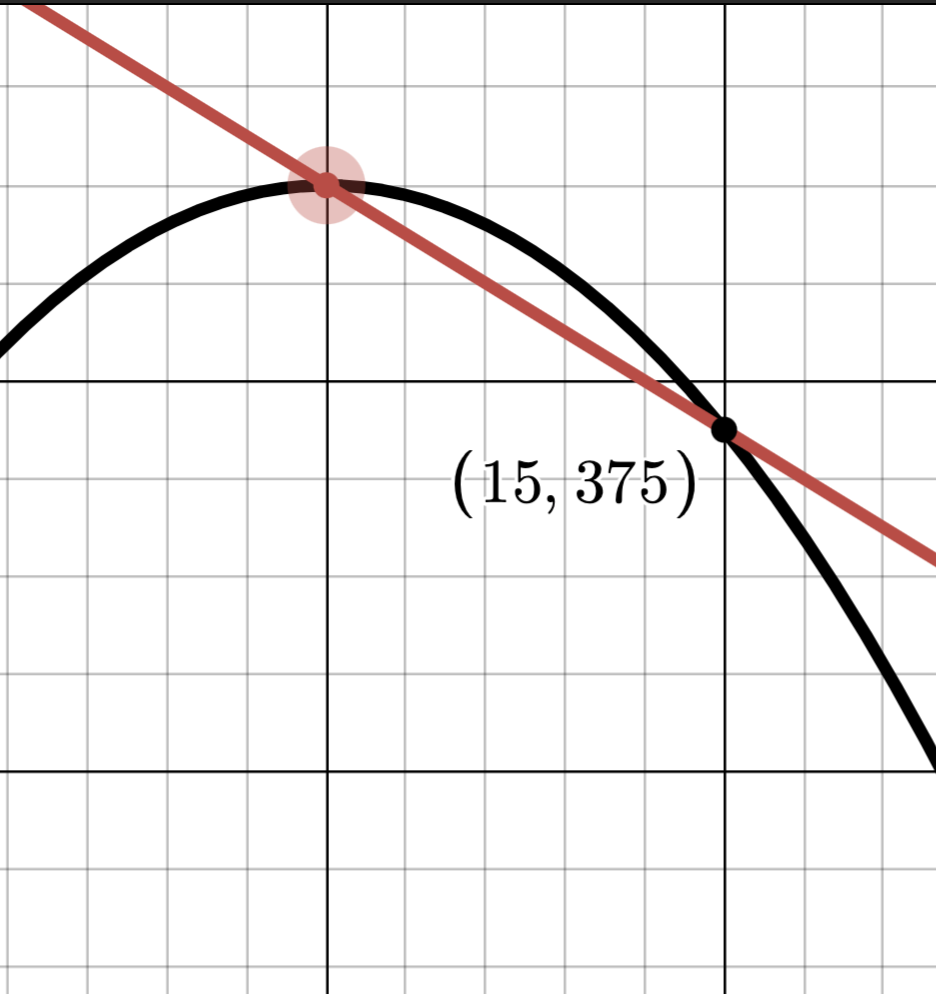
\includegraphics[width=2in]{./IntroductiontoDerivativesGraphics/sectotan01.png} &  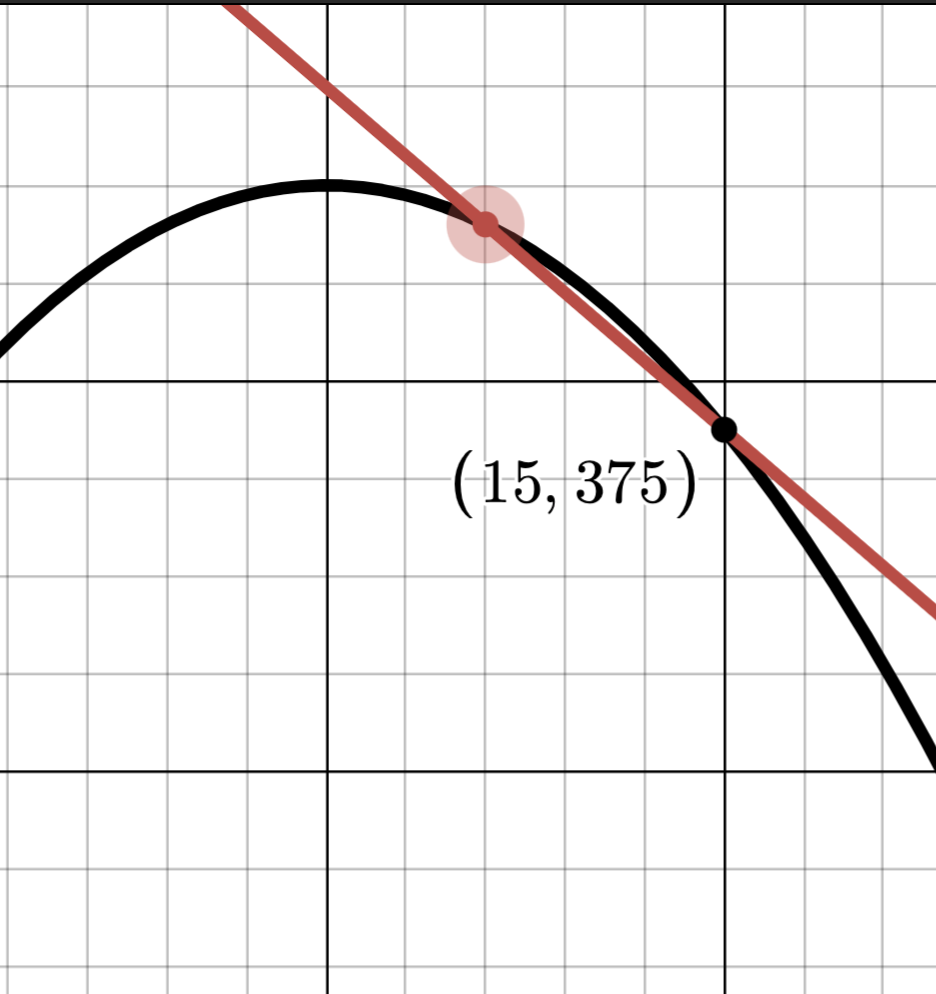
\includegraphics[width=2in]{./IntroductiontoDerivativesGraphics/sectotan03.png} &  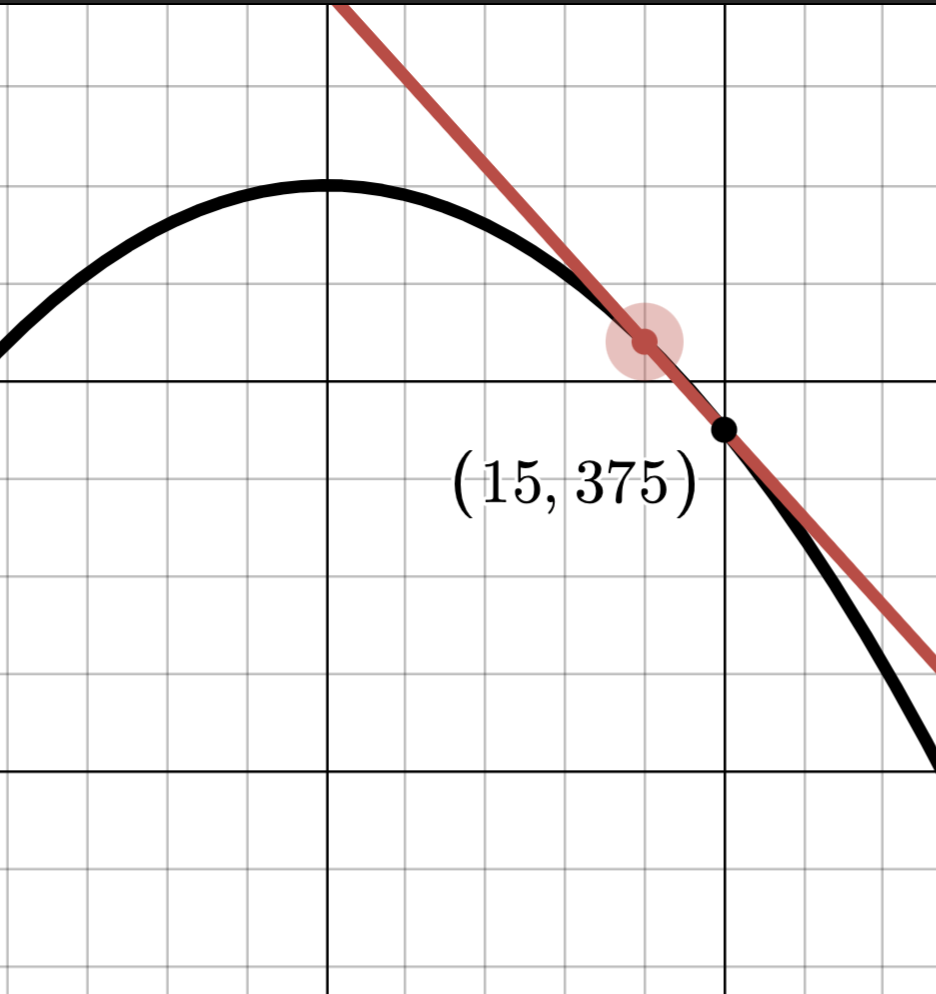
\includegraphics[width=2in]{./IntroductiontoDerivativesGraphics/sectotan05.png} \\
 
 
 \end{tabular}
 
 \end{center}
 To find the equation of the tangent line in this case, which we'll call $L(t)$,  we refer to the point-slope form of a line, Equation \ref{linearfunctionpointslope}:  \[ L(t) = s\left(t_{0} \right)+ m \left(t-t_{0} \right) = s(15) + v(15)(t-15) = 375 - 50(t-15) = -50t+1125.\]
 
The tangent line can best be thought of as `the best linear approximation' to the graph of $y = s(t)$ at $(15,375)$.  That is, if we zoom in near $(15,375)$, the graph of $y = s(t)$ and this tangent line become indistinguishable.  This property of $y = s(t)$ is called \index{local linearity}\textbf{local linearity} and is foundational to the analysis of functions.   Below we graph $y = s(t) =  -5t^2+100t$ along with $y = L(t) = -50t + 1125$ and observe the local linearity near $(15, 375)$. 
  
  \medskip

\begin{center}

\begin{tabular}{ccc}

 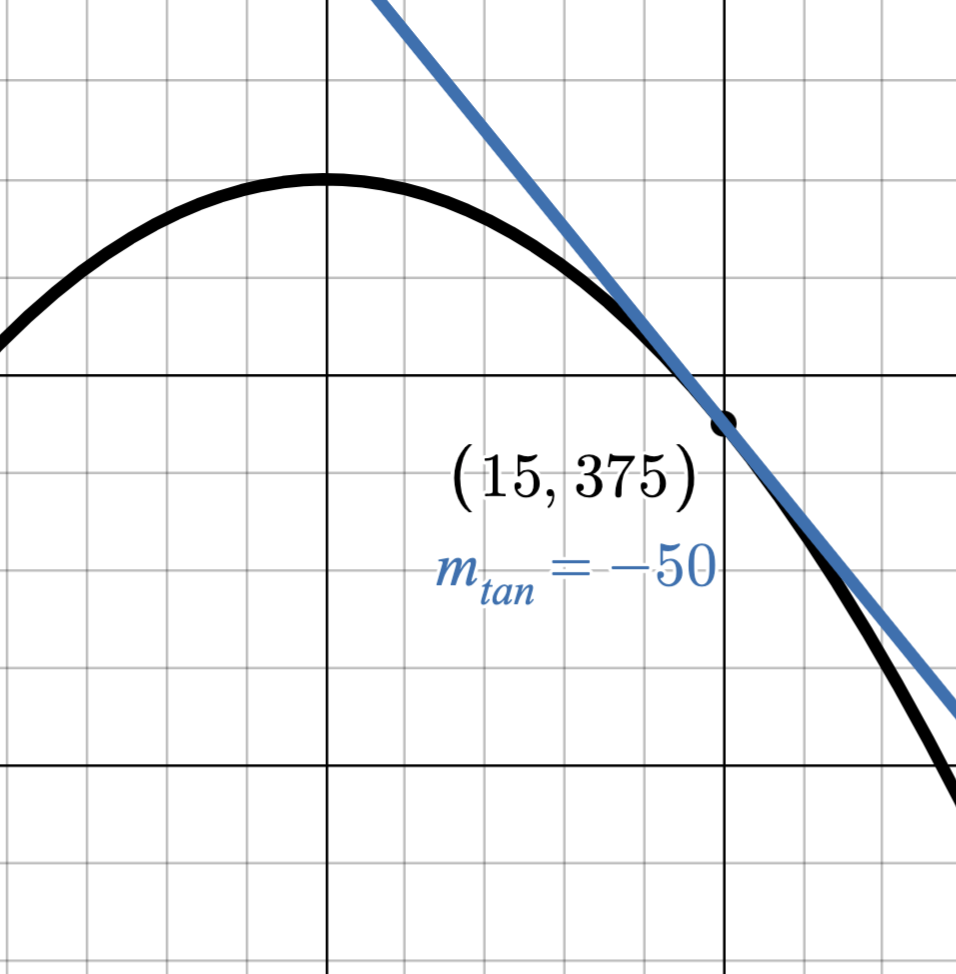
\includegraphics[width=2in]{./IntroductiontoDerivativesGraphics/tangent.png} &  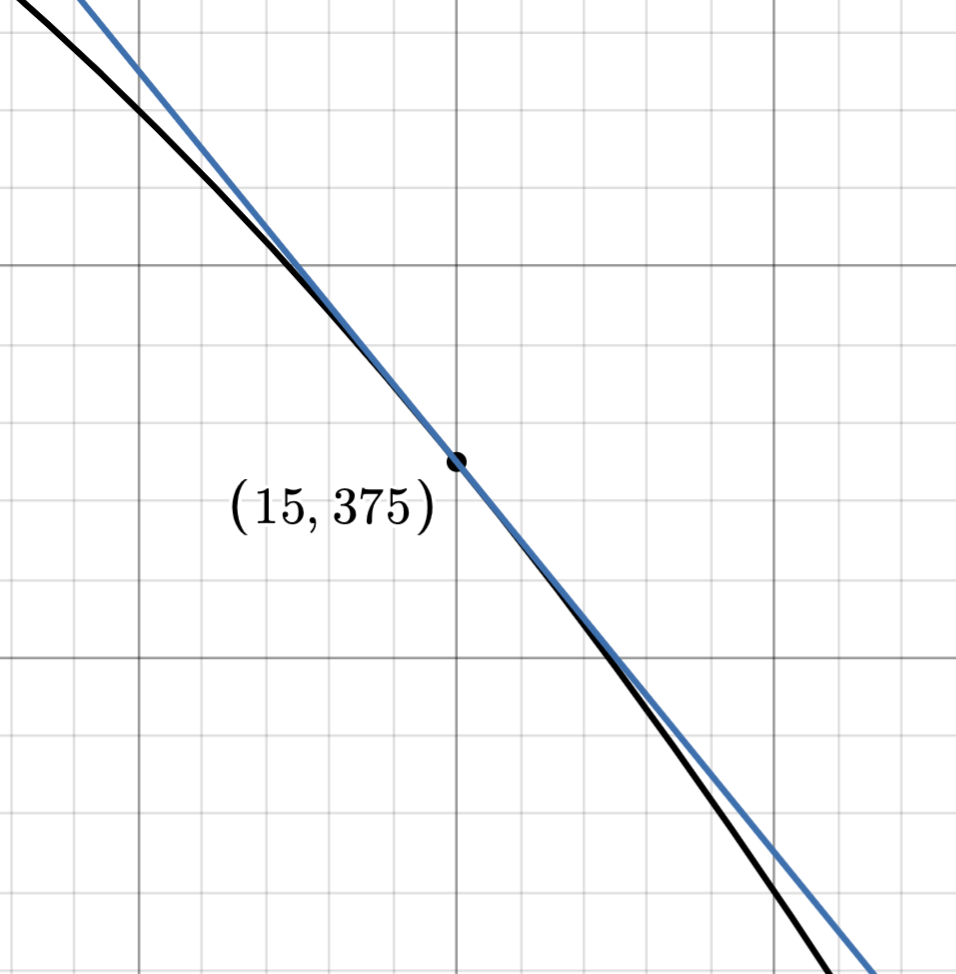
\includegraphics[width=2in]{./IntroductiontoDerivativesGraphics/tangentzoom1.png} &  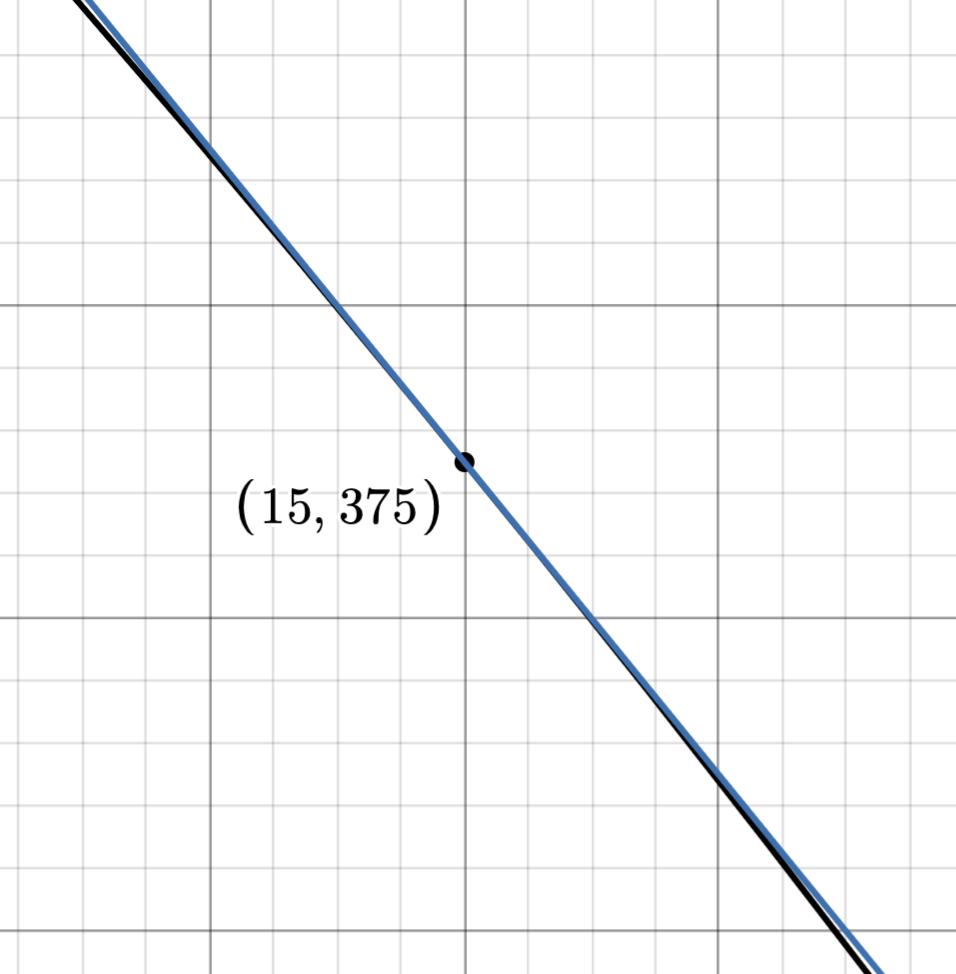
\includegraphics[width=2in]{./IntroductiontoDerivativesGraphics/tangentzoom2.png} \\
 
 The tangent line at $(15, 375)$. & Zooming in near $(15, 375)$. & Zooming in closer to $(15, 375)$. \\
 
 \end{tabular}
 
 \end{center}
 
Our next step is to generalize these notions to all functions.


\subsection{Difference Quotients and Derivatives}
\label{diffquotderiv}


Recall  in Section \ref{AverageRateofChange} the concept of the average rate of change of a function over the interval $[a,b]$  is the slope between the two points $(a, f(a))$ and $(b, f(b))$ and is given by \[ \dfrac{\Delta[f(x)]}{\Delta x} = \dfrac{f(b)-f(a)}{b-a}.\]

Geometrically, the average rate of change is the slope of the so-called \index{secant line}\textbf{secant line} which `cuts' through the graph of $y = f(x)$ at the points $(a,f(a))$ and $(b, f(b))$:

\begin{center}
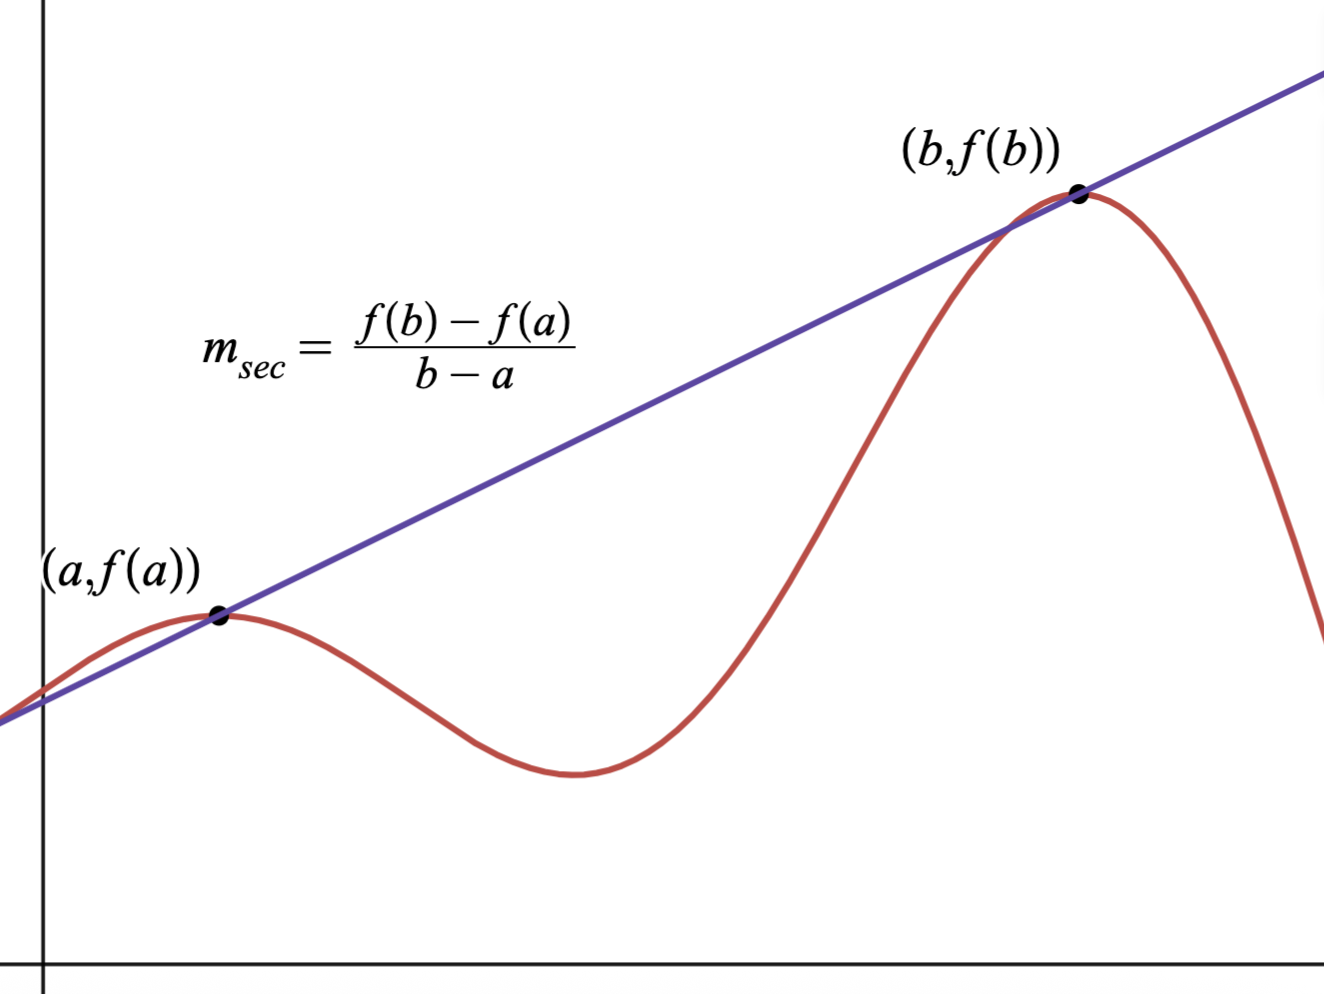
\includegraphics[width=4in]{./IntroductiontoDerivativesGraphics/SecantLine.png}
\end{center}

Consider a function $f$ defined over an interval containing $x$ and $x+h$ where $h \neq 0$. The average rate of change of $f$ over the interval $[x,x+h]$ is thus given by the formula:\footnote{assuming $h>0$;  otherwise, we  the interval is $[x+h, x]$.  We get the same formula for the difference quotient either way.}

\[ \dfrac{\Delta[f(x)]}{\Delta x} = \dfrac{f(x+h)-f(x)}{h}, \quad h \neq 0.\]

The above is an example of what is traditionally called the  \index{difference quotient}\textbf{difference quotient}  or  \textbf{Newton quotient} of $f$, since it is the \textit{quotient} of two \textit{differences}, namely $\Delta[f(x)]$ and $\Delta x$. Another formula for the difference quotient (as seen in Section \ref{rocarithmetic}) keeps with the notation $\Delta x$ instead of $h$:


\[ \dfrac{\Delta[f(x)]}{\Delta x} = \dfrac{f(x+\Delta x)-f(x)}{\Delta x}, \quad \Delta x \neq 0.\]


It is important to understand that in this formulation of the difference quotient, the variables `$x$' and `$\Delta x$' are distinct - that is they do not combine as like terms. 

\medskip


Note that, regardless of which form the difference quotient takes, when $h$,  $\Delta x$, or  $\Delta t$ is $0$, the difference quotient returns the indeterminate form `$\frac{0}{0}$.' As we've seen with rational functions in Section \ref{IntroRational}, when this happens, we can use a limit to help us \textbf{determine} the \textbf{indeterminate} form.  

\medskip

In Section \ref{avginstantvelocity}, taking the limit of average velocity as $\Delta t \rightarrow 0$  produced instantaneous velocity.  More generally, taking the limit of the average rate of change  as the denominator approaches $0$ produces the \index{instantaneous rate of change}\index{rate of change ! instantaneous}\textbf{instantaneous rate of change} of the function at that point.   The instantaneous rate of change of a function is called the \index{derivative}\textbf{derivative} of the function is defined below.

\medskip


\colorbox{ResultColor}{\bbm

\begin{defn} \label{derivativedefn} Given a function $f$ defined on an open interval containing $x=a$, the \textbf{derivative} of $f$ at $a$, denoted $f'(a)$ is defined as

\[ f'(a) = \lim_{h \rightarrow 0} \dfrac{f(a+h) - f(a)}{h}, \quad \text{provided this limit exists.} \]

 The number $f'(a)$ represents the \index{instantaneous rate of change}\index{rate of change ! instantaneous}\textbf{instantaneous rate of change} of $f$ with respect to $x$ at the input $x = a$.  If $f'(a)$ exists, we say $f$ is \index{differentiable}\textbf{differentiable} at $x = a$.

\end{defn}

\ebm}

\medskip

Using the language of derivatives, Examples \ref{averagevelocityrocketex}  and \ref{averagevelocityrocketexreprise} have us computing $v(15) = s'(15)$.   Moreover, since the derivative is a rate of change, it's important to note that the associated units of $f'(a)$ are $\frac{ \text{units of $f(x)$}}{\text{units of $x$}}$.  This tracks with the units of  $v(15) = s'(15)$ being $\frac{ \text{feet}}{\text{second}}$, a velocity.

\medskip

As in Section \ref{avginstantvelocity},  $f'(a)$ represents the slope of the tangent line at the point $(a, f'(a))$.  We use this to formally define the \index{tangent line}\index{line ! tangent}\textbf{tangent line} below.

\medskip


\colorbox{ResultColor}{\bbm

\begin{defn} \label{tangentlinedefn}  If $f$ is differentiable at $x = a$, then $f'(a) =  m_{\text{tan}}$, the slope of the \index{tangent line}\index{line ! tangent}\textbf{tangent line}\textbf{tangent line} to $y = f(x)$ at $(a, f(a))$.   The equation of the tangent line is therefore:  $y = f'(a)(x-a) + f(a)$.  



\end{defn}

\ebm}

\medskip

We put these definitions to good use in the following example.

\pagebreak

\begin{ex}  \label{tangentlineex}  Let $f(x) = -x^2 + 3x-1$.  

\begin{enumerate}

\item Find the equation of the tangent line to $y = f(x)$ at $x = -2$.  Check your answer graphically.

\item  If $f$ represents the temperature (in degrees Celsius) $x$ hours after Noon on a particular day, interpret $f'(-2)$ in terms of time and temperature.

\end{enumerate}

\bigskip

{\bf Solution.}  \begin{enumerate} \item We first find $m_{\text{tan}} = f'(-2)$ using Definition \ref{derivativedefn} with $a = -2$:  $ f'(-2) = \ds{\lim_{h \rightarrow 0} \dfrac{f(-2+h) - f(-2)}{h}}$. 

First we find $f(-2+h)$ and are  careful to apply the exponent in the expression $-(-2+h)^2$ first:

\[ \begin{array}{rclr}  
  f(-2+h) & = & -(-2+h)^2 +3(-2+h) -1 & \\ 
  & = & - (4 - 4h+h^2) -6+3h-1 & \\
 & = & -4 + 4h-h^2-6+3h-1& \\
  & = & -h^2+7h-11& \\
 \end{array} \]

Next, we find $f(-2) = -(-2)^2 + 3(-2)-1 = -11$, so the difference quotient is:

\[ \begin{array}{rclr}

\dfrac{f(-2+h)-f(-2)}{h} & = & \dfrac{(-h^2+7h-11) -(-11)}{h} & \\[8pt]
                                & = & \dfrac{-h^2+7h}{h} & \text{simplify}\\[8pt]
                                & = &  \dfrac{h(-h+7)}{h} & \text{factor} \\[8pt]
                                & = &  \dfrac{\cancel{h}(-h+7)}{\cancel{h}} &  \text{cancel} \\[8pt]
                                & = & -h+7\\ \end{array} \]



Finally, we get $ f'(-2) = \ds{\lim_{h \rightarrow 0} \dfrac{f(-2+h) - f(-2)}{h} = \lim_{h \rightarrow 0} (-h+7) = -(0) + 7 = 7}$.

\bigskip

Hence, the slope of the tangent line is $m_{\text{tan}} = f'(-2) = 7$.  Hence, the equation of the tangent line is: 

\[ \begin{array}{rclr}  
 y & = & f'(-2)(x - (-2)) + f(-2) & \\ 
  & = & 7(x+2) - 11 & \\
 & = & 7x+14 - 11& \\
  y & = & 7x+3& \\
 \end{array} \]

Graphing $y = 7x+3$ and $y = f(x)$ near $(-2,-11)$ reveals the local linearity we would expect:

\begin{center}

\begin{tabular}{cc}

 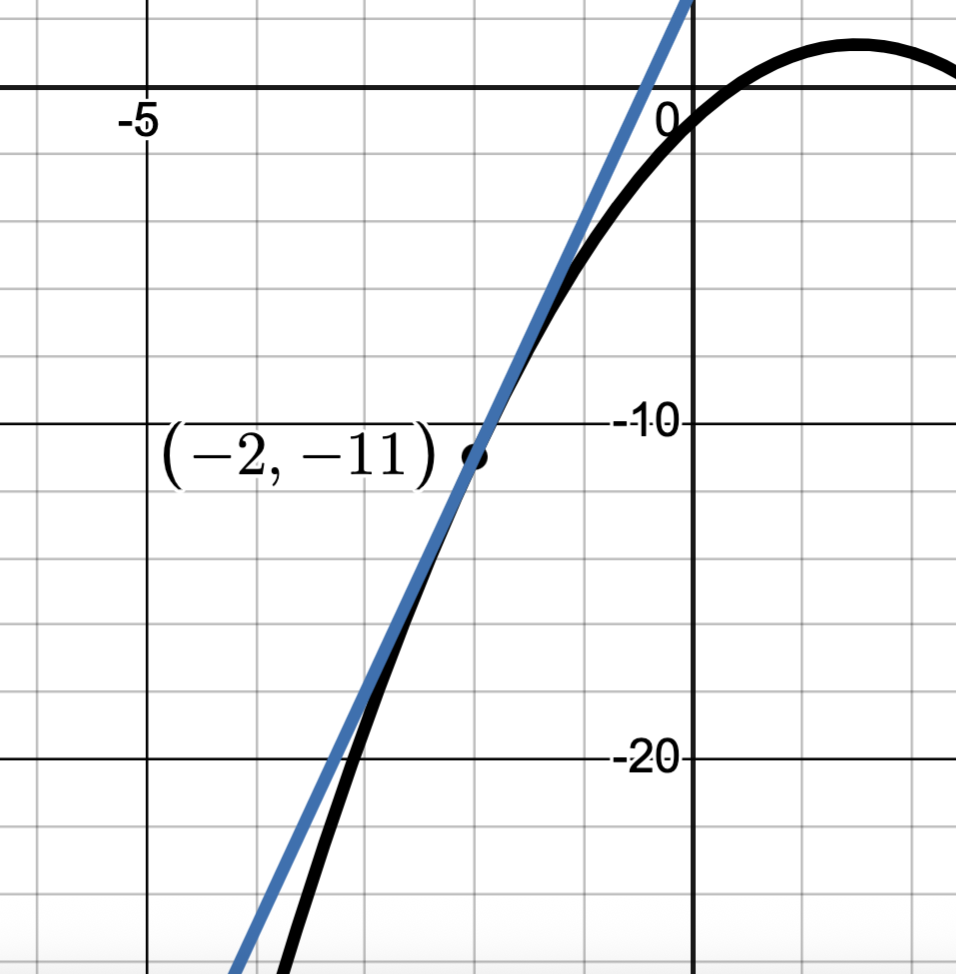
\includegraphics[width=2.5in]{./IntroductiontoDerivativesGraphics/TLEx.png} &  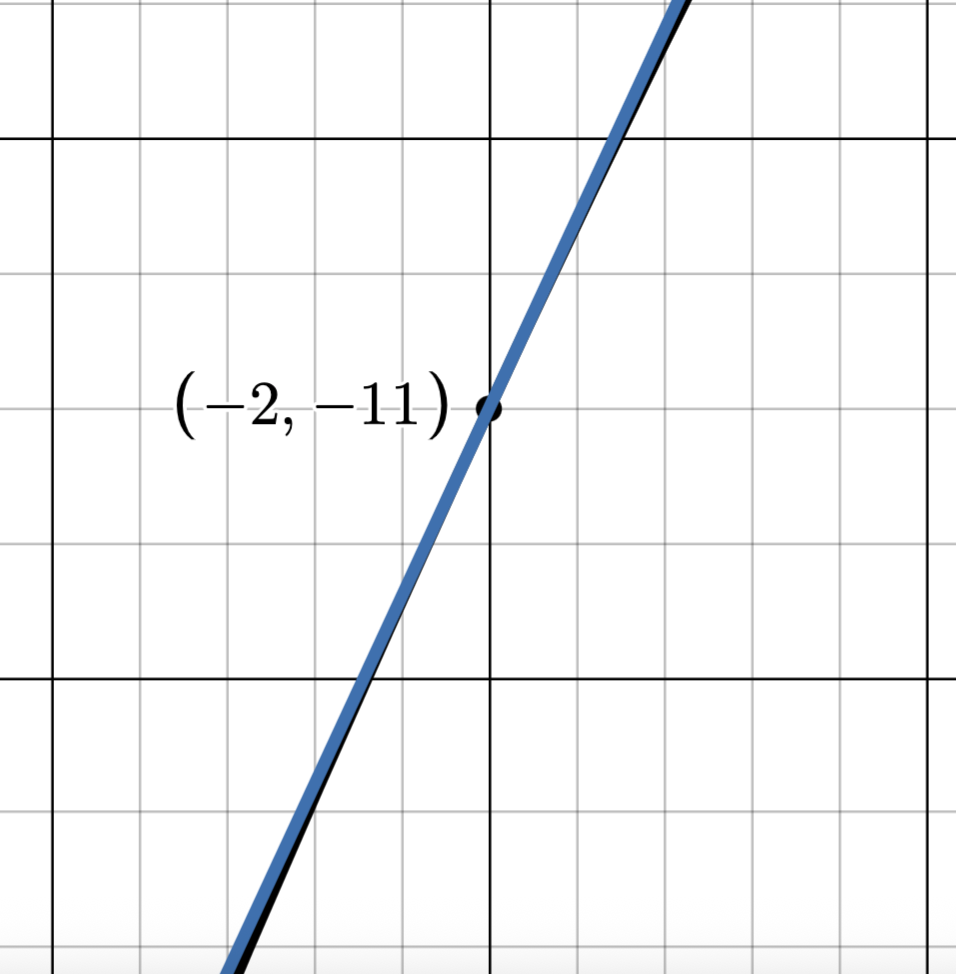
\includegraphics[width=2.5in]{./IntroductiontoDerivativesGraphics/TLExZoom.png}  \\
 
 The tangent line at $(-2,-11)$. & Zooming in near $(-2, -11)$.  \\
 
 \end{tabular}
 
 \end{center}
 
 \item Since $x$ represents the number of hours \textbf{after} Noon, $x = -2$ corresponds to $2$ hours \textbf{before} Noon, or 10 AM.  Since the units of $f(x)$ are degrees Celsius and the units of $x$ are hours, the units of $f'(-2)$ are degrees Celsius per hour.  Since $f'(-2)$ is positive, we know the slope is positive, so the temperature is increasing.  Putting all this together,   $f'(-2) = 7$ means that at 10 AM, the temperature is rising at a rate of $7$ degrees Celsius  per hour. \hfill \qed
 
 \end{enumerate}



\end{ex}

What if we wanted to find the equation of the tangent line to the graph of the function in Example \ref{tangentlineex}  at $x = 0$?  $x = 1$?  $x = 5$?  We'd ostensibly need to run through difference quotients and limit calculations for each and every input value: $x = 0$, $x = 1$, and $x = 5$.  Or we could do a single limit with a generic `$x$', simplify the difference quotient and take the limit once, and substitute in particular values of $x$:

\medskip

\colorbox{ResultColor}{\bbm

\begin{defn} \label{derivativefcndefn} Given a function $f$ defined on an open interval, the \textbf{derivative} of $f$, denoted  $f'(x)$ is the function

\[ f'(x) = \lim_{h \rightarrow 0} \dfrac{f(x+h) - f(x)}{h}, \quad \text{provided the limit exists.}\]

\end{defn}

\ebm}

\medskip

It is worth noting that if we set $h = \Delta x$, and consider the graph $y = f(x)$, we get:  \[ f'(x) = \lim_{h \rightarrow 0} \dfrac{f(x+h) - f(x)}{h} = \lim_{\Delta x \rightarrow 0} \dfrac{f(x+\Delta x) - f(x)}{\Delta x}  = \lim_{\Delta x \rightarrow 0} \dfrac{\Delta [f(x)] }{\Delta x} =  \lim_{\Delta x \rightarrow 0} \dfrac{\Delta y }{\Delta x} ,\] which is why sometimes the derivative is denoted\footnote{This is the so-called  \href{https://en.wikipedia.org/wiki/Gottfried_Wilhelm_Leibniz}{\underline{Leibniz}} notation \ldots}  $\frac{dy}{dx}$.

\pagebreak


\begin{ex}  \label{derivativeex}  Let $f(x) = -x^2 + 3x-1$.  

\begin{enumerate}

\item \label{firstpart} Find an expression for $f'(x)$.  

\item  Find $f'(-2)$ using your answer to part \ref{firstpart}   and compare that to what you obtained in Example \ref{tangentlineex}.

\item  Find the equation of the tangent line to the graph of $y = f(x)$ at $x = 0$.  Check your answer graphically.

\item  Solve $f'(x) = 0 $ and interpret your answer graphically.

\end{enumerate}

\bigskip

{\bf Solution.}

\begin{enumerate}

\item  We start finding $f'(x) = \ds{ \lim_{h \rightarrow 0} \dfrac{f(x+h) - f(x)}{h}}$ by first finding $f(x+h)$:

\[ \begin{array}{rclr}  
  f(x+h) & = & -(x+h)^2 +3(x+h) -1 & \\ 
  & = & - (x^2 +2xh+h^2) +3x+3h-1 & \\
 & = & -x^2 -  2xh - h^2+3x+3h-1& \\
 \end{array} \]

The difference quotient simplifies as follows:

\[ \begin{array}{rclr}

\dfrac{f(x+h)-f(x)}{h} & = & \dfrac{( -x^2 - 2xh - h^2+3x+3h-1) -(-x^2+3x-1)}{h} & \\[8pt]
                                & = & \dfrac{-x^2 - 2xh - h^2+3x+3h-1 + x^2-3x+1}{h} & \\[8pt]
                                 & = & \dfrac{-2xh-h^2+3h}{h} & \text{simplify}\\[8pt]
                                & = &  \dfrac{h(-2x - h + 3)}{h} & \text{factor} \\[8pt]
                                & = &  \dfrac{\cancel{h}(-2x-h+3)}{\cancel{h}} &  \text{cancel} \\[8pt]
                                & = & -2x-h+3\\ \end{array} \]

Our last step is to take the limit:   $f'(x) = \ds{ \lim_{h \rightarrow 0} \dfrac{f(x+h) - f(x)}{h} = \lim_{h \rightarrow 0} (-2x-h+3)}$.  Notice here that we have two variables, $x$ and $h$, in the limit.  Of these two variables, we are taking the limit on the $h$:  $h \rightarrow 0$.  As far as $h$ is concerned, $x$ may as well be just another constant like the `$3$'.  Hence, $f'(x) = \ds{ \lim_{h \rightarrow 0} (-2x-h+3)}=  -2x - 0 + 3 = -2x+3$.

\item  Evaluating our formula for $f'(x)$ at $x = -2$ gives $f'(-2) = -2(-2) + 3 = 7$ which matches with what we obtained in Example \ref{tangentlineex}.

\item The equation of the tangent line to the graph of $y = f(x)$ at $x = 0$ is $y = f'(0) (x - 0) + f(0)$.  We have $f'(0)=2(0) + 3 = 3$ and $f(0) = -(0)^2+3(0)-1 = -1$.  We get $y = 3(x-0)+(-1)$ so $y = 3x-1$. Our graph bears this out.

\begin{center}

\begin{tabular}{cc}

 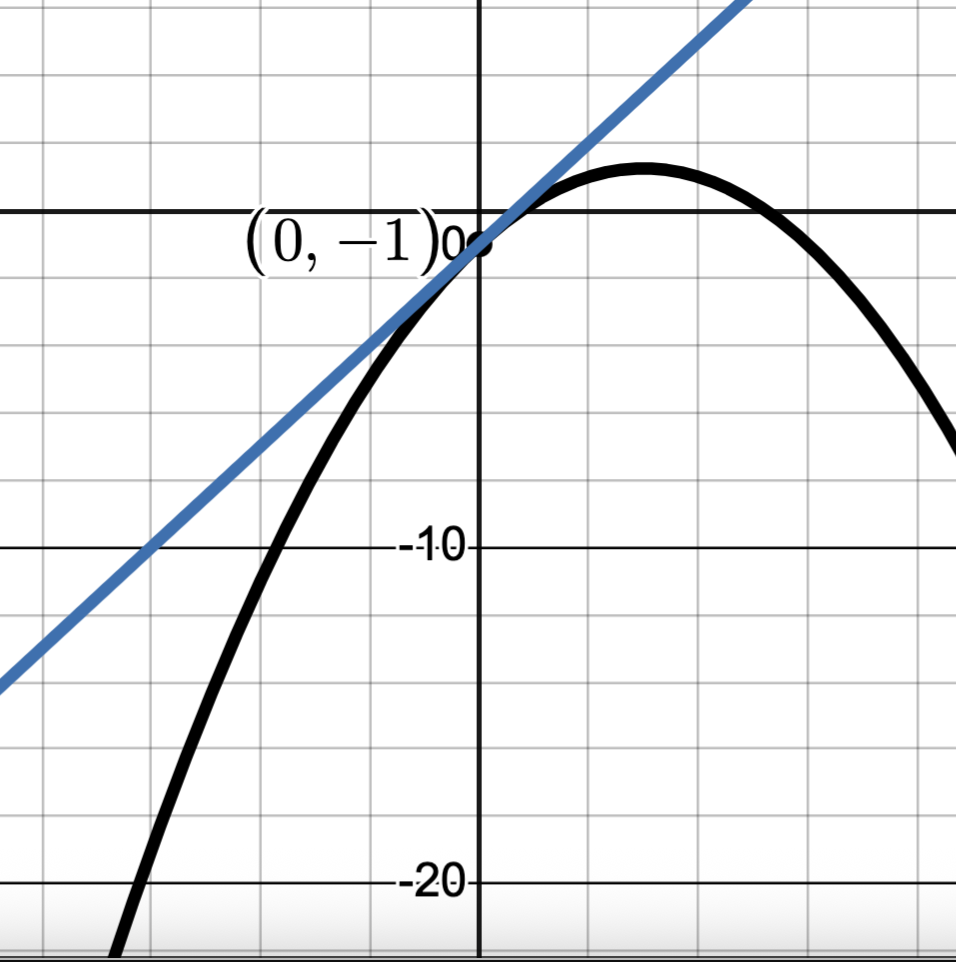
\includegraphics[width=2.5 in]{./IntroductiontoDerivativesGraphics/TL02.png} &  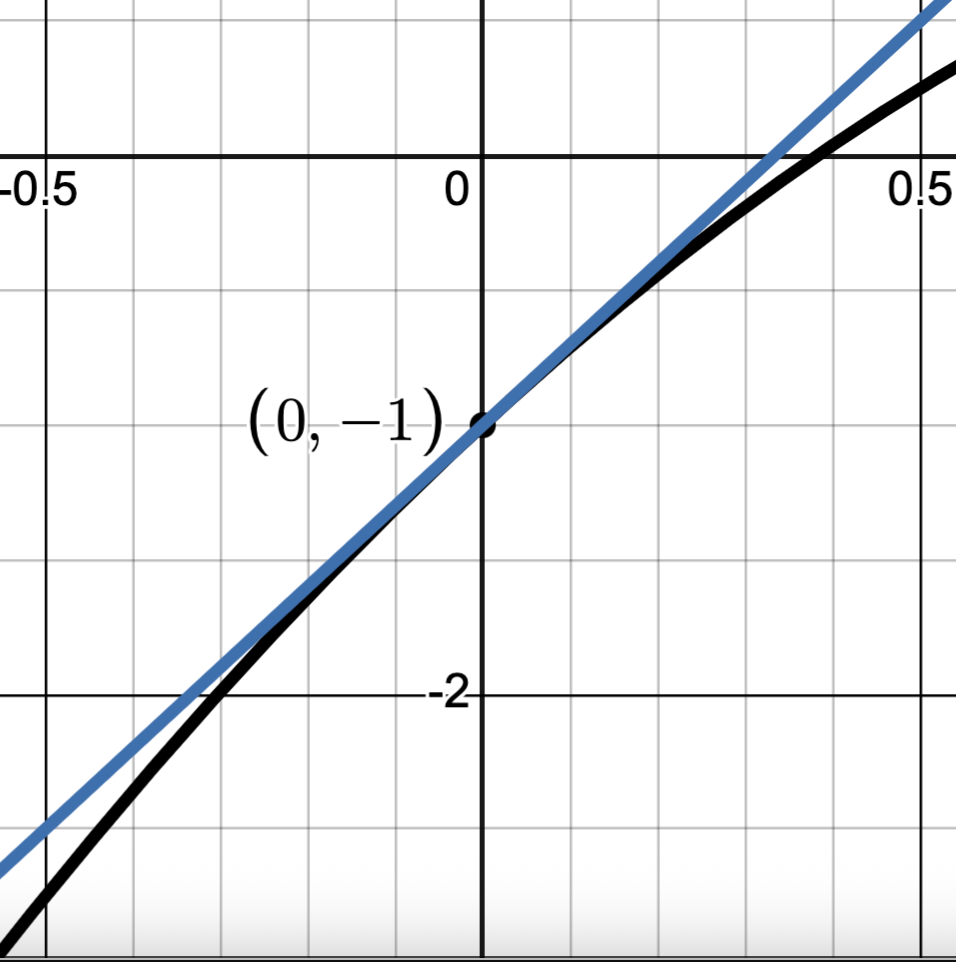
\includegraphics[width=2.5in]{./IntroductiontoDerivativesGraphics/TL02Zoom.png}  \\
 
 The tangent line at $(0,-1)$. & Zooming in near $(0, -1)$.  \\
 
 \end{tabular}
 
 \end{center}
 
 \item  Solving $f'(x) = 0$ gives $-2x+3 = 0$ so $x = \frac{3}{2}$.  This means the slope of the tangent line at the point $\left(\frac{3}{2}, f\left(\frac{3}{2}\right) \right)$ is $0$, so the tangent line there is horizontal.  We find 
 $f\left(\frac{3}{2}\right) = -\left( \frac{3}{2}\right)^2 + 3\left(\frac{3}{2}\right) - 1 = \ldots = \frac{5}{4}$.  Hence, the tangent line at  $\left(\frac{3}{2}, \frac{5}{4} \right)$ is $y = \frac{5}{4}$.  Graphically, this checks out.
 
 
 
\begin{center}

\begin{tabular}{cc}

 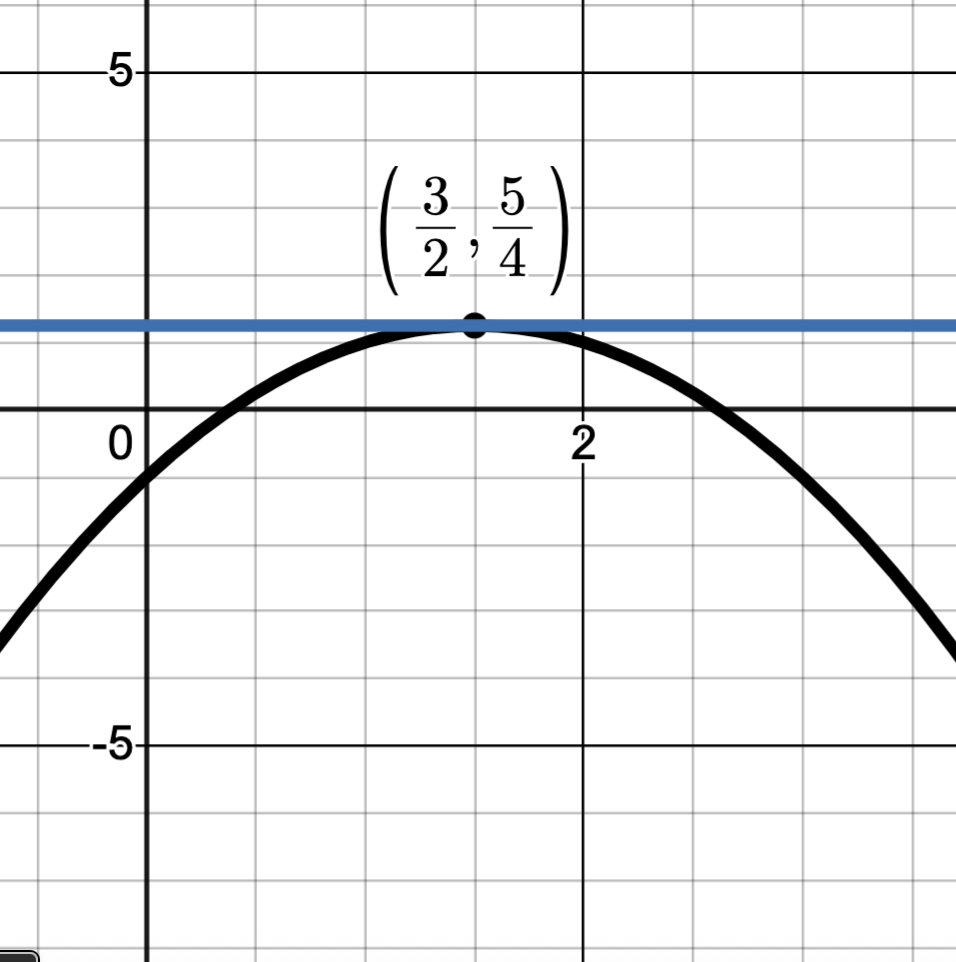
\includegraphics[width=3in]{./IntroductiontoDerivativesGraphics/HTL.png} &  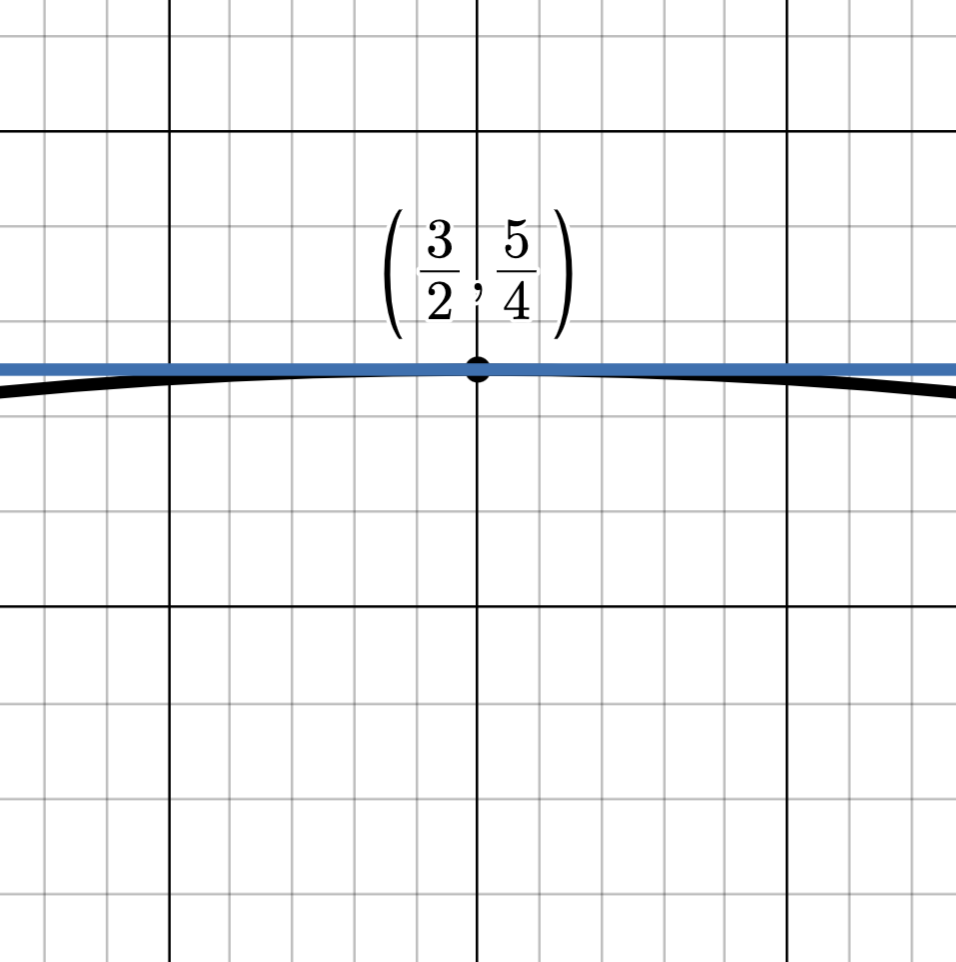
\includegraphics[width=3in]{./IntroductiontoDerivativesGraphics/HTLZoom.png}  \\
 
 The tangent line at  $\left(\frac{3}{2}, \frac{5}{4} \right)$. & Zooming in near $\left(\frac{3}{2}, \frac{5}{4} \right)$.  \\
 
 \end{tabular}
 
 \end{center}
 
 \hfill \qed


\end{enumerate}

\end{ex}

The astute reader will note that the graph of $f(x) = -x^2+3x-1$ in Example \ref{derivativeex} is a parabola and finding where $f'(x) = 0$ lead us right back to the vertex.  Using a derivative to find the vertex may seem a bit excessive given that we've algebraically derived a handy `vertex formula' in Section \ref{QuadraticFunctions}.   However, as the functions we aim to analyze become more and more sophisticated, the tools we use to analyze them must also become more sophisticated.  The derivative is one such tool that has a near universal application.\footnote{As we'll see in Section \ref{DerivativeAnalysis}.}

\medskip



\begin{ex}  \label{morederivativesex} $~$

\begin{enumerate}

\item  For $f(x) = x^2-x-2$, find and simplify:   



\begin{enumerate}

\item  $f'(3)$ %$\dfrac{f(3+h)-f(3)}{h}$ 

\item  The equation of the tangent line to the graph $y = f(x)$ at $(3, f(3))$.  

Check your answer graphically.

\item  $f'(x)$ %$\dfrac{f(x+h)-f(x)}{h}$.

\end{enumerate}



\item  For $g(x) = \dfrac{3}{2x+1}$, find and simplify:\footnote{A review of Section \ref{AppRatExpEqus} may be in order for this problem.}



\begin{enumerate}

\item  $g'(0)$ %$\dfrac{g(\Delta x)-g(0)}{\Delta x}$

\item  The equation of the tangent line to the graph $y = g(x)$ at $(0, g(0))$.  

Check your answer graphically.
 
\item  $g'(x)$ %$\dfrac{g(x+\Delta x)-g(x)}{\Delta x}$.

\end{enumerate}




\item  $r(t) = \sqrt{t}$,  find and simplify:\footnote{A review of Section \ref{rationalizingdenomandnumer} may be in order for this problem.}

\begin{enumerate}

\item $r'(9)$ %$\dfrac{r(9+\Delta t)-r(9)}{\Delta t}$ 

\item  The equation of the tangent line to the graph $y = r(t)$ at $(9, r(9))$.

 Check your answer graphically.


 \item $r'(t)$ %$\dfrac{r(t+\Delta t)- r(t)}{\Delta t}$.
 
 \end{enumerate}

\end{enumerate}



{\bf Solution.}
 
\begin{enumerate}

\item \begin{enumerate} \item To find $f'(3) = \ds{\lim_{h \rightarrow 0}}$ $\frac{f(3+h)-f(3)}{h}$ we first simplify $f(3+h)$:

\[ \begin{array}{rclr}  
  f(3+h) & = & (3+h)^2 - (3+h) -2 & \\ 
  & = & 9 + 6h+h^2 - 3 - h -2 & \\
 & = & 4 + 5h + h^2 & \\
 \end{array} \]

Since $f(3) = (3)^2-3-2 = 4$, we get for the difference quotient:

\[ \begin{array}{rclr}

\dfrac{f(3+h)-f(3)}{h} & = & \dfrac{(4 + 5h + h^2) -4}{h} & \\[8pt]
                                & = & \dfrac{5h+h^2}{h} & \\[8pt]
                                & = &  \dfrac{h(5+h)}{h} & \text{factor} \\[8pt]
                                & = &  \dfrac{\cancel{h}(5+h)}{\cancel{h}} & \text{cancel}\\[8pt]
                                & = & 5+h \\ \end{array} \]
 Hence, $f'(3) = \ds{\lim_{h \rightarrow 0} (5+h) = 5+0 = 5}$.
 
 
 \item  The equation of the tangent line at $x = 3$ is:  $y = f'(3)(x-3) + f(3) = 5(x-3) + 4$, or $y = 5x-11$. We check graphically below.
 
 \begin{center}

 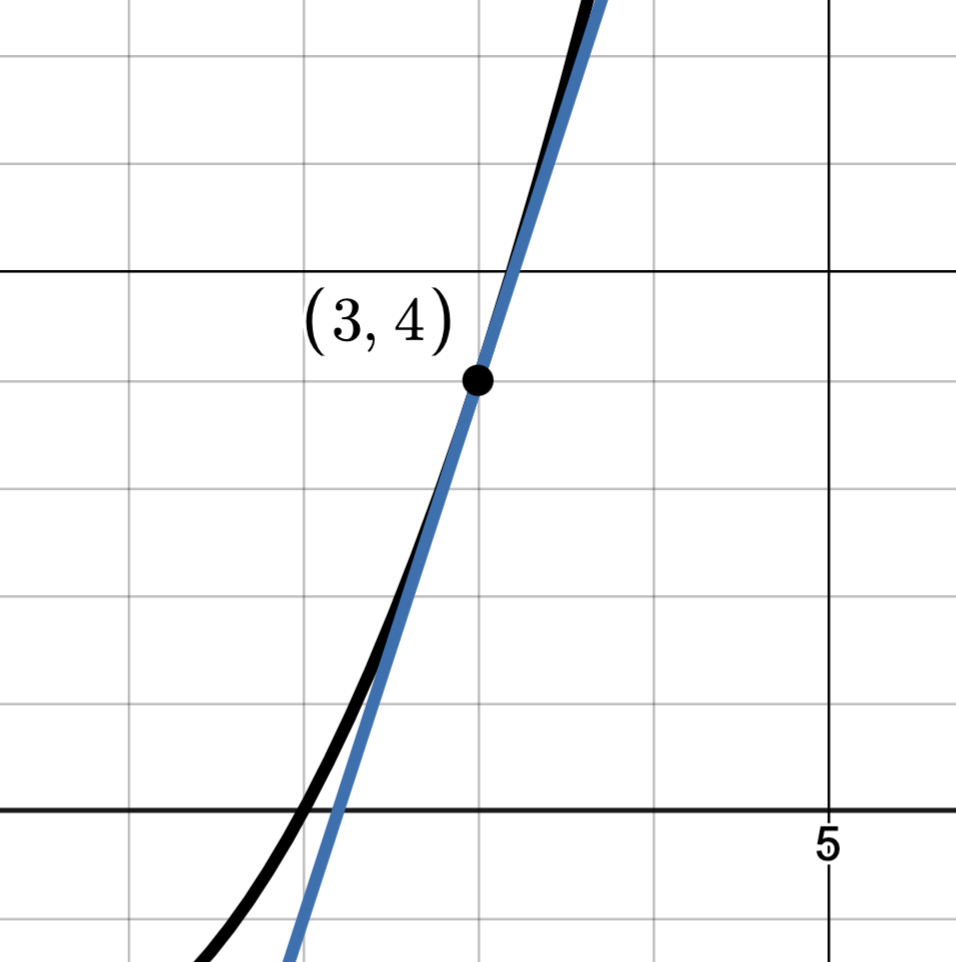
\includegraphics[width=2in]{./IntroductiontoDerivativesGraphics/TLEx201.png} 
 
 $y = f(x)$ and  $y = 5x-11$  near $(3,4)$  

 \end{center}

 \item To find $f'(x) = \ds{\lim_{h \rightarrow 0}}$ $\frac{f(x+h)-f(x)}{h}$, we first find $f(x+h)$:


\[ \begin{array}{rclr}  
 
 f(x+h) & = & (x+h)^2 - (x+h) -2 & \\ [8pt]
 & = & x^2 + 2xh + h^2 - x - h - 2.
 \end{array} \]

So the difference quotient is

\setlength{\extrarowheight}{12pt}

\begin{longtable}{rclr}  

$\dfrac{f(x+h)-f(x)}{h}$ & = & $\dfrac{\left(x^2+2xh+h^2-x-h-2 \right)-\left(x^{2}-x-2 \right)}{h}$ & \\[8pt] 
& = & $\dfrac{x^2+2xh+h^2-x-h-2-x^2+x+2}{h}$ & \\[8pt]
& = & $\dfrac{2xh+h^2-h}{h}$ & \\[8pt]
& = & $\dfrac{h \left(2x+h-1\right)}{h}$ & factor \\[8pt]
& = & $\dfrac{\cancel{h} \left(2x+h-1\right)}{\cancel{h}}$ & cancel \\[8pt]
& = & $2x+h-1$. \\

\end{longtable} 

Hence, $f'(x) = \ds{\lim_{h \rightarrow 0} (2x+h-1) = 2x + 0 - 1}$ so $f'(x) = 2x-1$. Note that using this formula, we get  $f'(3) = 2(3)-1 = 5$ which checks our answer above.


\end{enumerate}

\item  \begin{enumerate} \item Next we find  $g'(0) = \ds{\lim_{h \rightarrow 0}}$$\frac{g(0+h)-g(0)}{h}  = \frac{g(h) - g(0)}{h}$.

Since $g(h) = \frac{3}{2 h + 1}$ and $g(0) = \frac{3}{2(0)+1} = 3$, our difference quotient contains a complex fraction.  Thinking ahead, we need to (eventually) be able to cancel the factor `$h$' from the denominator $\frac{g(h) - g(0)}{h}$, so we begin by simplifying the complex fraction and see where that takes us:

\begin{longtable}{rclr}  

$\dfrac{g(0+h)-g(0)}{h}$ & = & $\dfrac{\dfrac{3}{2h+1}-3}{h}$ & \\[10pt]
& = &  $\dfrac{\dfrac{3}{2h+1}-3}{h} \cdot \dfrac{(2h+1)}{(2h+1)}$ & \\[10pt]
& = &  $\dfrac{3-3(2h+1)}{h(2h+1)}$  & \\[10pt]
& = &  $\dfrac{3 - 6 h - 3}{h(2h+1)}$  & \\[10pt]
& = &  $\dfrac{-6h}{h(2h+1)}$  & \\[10pt]
& = &  $\dfrac{-6\cancel{h}}{\cancel{h}(2h+1)}$  & \text{cancel} \\[10pt]
& = &  $\dfrac{-6}{2h+1}$.  & \\ 

\end{longtable}

We are now ready to take the limit:  \[g'(0) = \lim_{h \rightarrow 0} \frac{-6}{2h+1} = \frac{-6}{2(0)+1} = -6.\]

\item The equation of the tangent line when $x = 0$ is: $y = g'(0)(x-0) + g(0) = (-6)(x-0)+ 3$ or $y = -6x+3$, which checks graphically below.

 \begin{center}

 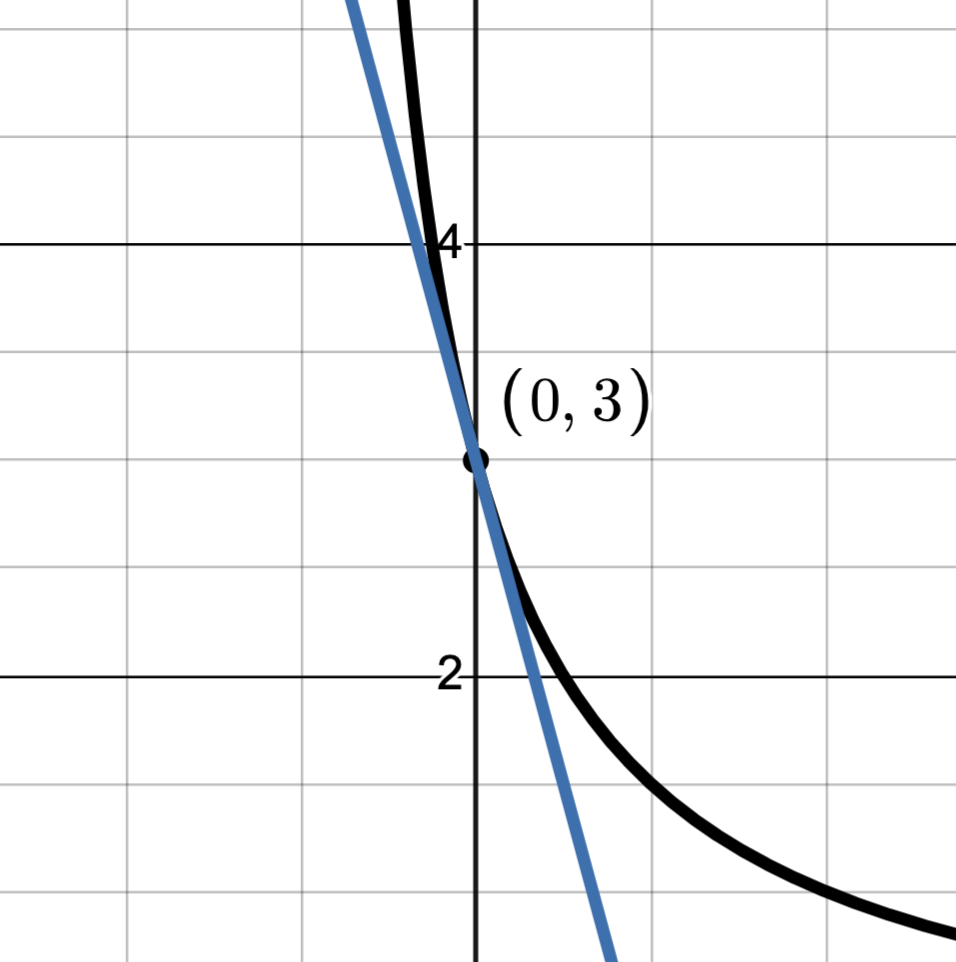
\includegraphics[width=2in]{./IntroductiontoDerivativesGraphics/TLEx202.png} 
 
 $y = g(x)$ and  $y =-6x+3$  near $(0,3)$  

 \end{center}



\item To find $g'(x)$, we first find $g(x+h)$:

 \[ \begin{array}{rclr}  
 g(x+h) & = & \dfrac{3}{2(x+h)+1} & \\[10pt]
 & = & \dfrac{3}{2x+2h+1} \\
 \end{array} \]

Simplifying the difference quotient involves simplifying the resulting complex fraction, as above, keeping an eye out for an opportunity to cancel the factor `$h$' from the denominator:

\begin{longtable}{rclr}  

$\dfrac{g(x+h)-g(x)}{h}$ & = & $\dfrac{\dfrac{3}{2x+2h+1}-\dfrac{3}{2x+1}}{h}$ & \\[10pt]
& = &  $\dfrac{\dfrac{3}{2x+2h+1}-\dfrac{3}{2x+1}}{h} \cdot \dfrac{(2x+2h+1)(2x+1)}{(2x+2h+1)(2x+1)}$ & \\[10pt]
& = &  $\dfrac{3(2x+1)-3(2x+2h+1)}{h(2x+2h+1)(2x+1)}$  & \\[10pt]
& = &  $\dfrac{6x+3-6x-6h-3}{h(2x+2h+1)(2x+1)}$  & \\[10pt]
& = &  $\dfrac{-6h}{h(2x+2h+1)(2x+1)}$  & \\[10pt]
& = &  $\dfrac{-6\cancel{h}}{\cancel{h}(2x+2h+1)(2x+1)}$  & \text{cancel} \\[10pt]
& = &  $\dfrac{-6}{(2x+2h+1)(2x+1)}$.  & \\ 

\end{longtable}

Hence, \[g'(x) = \lim_{h \rightarrow 0} \frac{-6}{(2x+2h+1)(2x+1)} = \frac{-6}{(2x + 2(0) +1)(2x+1)} = - \frac{6}{(2x+1)^2}. \]   We check $g'(0) = -\frac{6}{(2(0)+1)^2} = \ldots = -6$, as required.

\end{enumerate}



\item \begin{enumerate} \item To find $r'(9) = \ds{\lim_{h \rightarrow 0}}$$\frac{r(9+h) - r(9)}{h}$, we start with $r(9+h) = \sqrt{9+h}$ and $r(9) = \sqrt{9} = 3$. Hence  our difference quotient is:

\[ \dfrac{r(9+h)-r(9)}{h} = \dfrac{\sqrt{9+h} - 3}{h}.\]


In order for us to determine the limit as $h \rightarrow 0$, we need to somehow cancel the factor of $h$ from the  \textbf{denominator}.  To do so,  we set about \textbf{rationalizing the numerator} by multiplying both numerator and denominator by the conjugate\footnote{Again, see Section  \ref{rationalizingdenomandnumer} for a review of these sorts of machinations.}of the numerator, $\sqrt{9+h} - 3$:


\[ \begin{array}{rcll}  

\dfrac{r(9+h) - r(9)}{h} & = & \dfrac{\sqrt{9+h} - 3}{h} & \\[15pt]
												
												 & = & \dfrac{\left(\sqrt{9+h} - 3 \right)}{h} \cdot \dfrac{\left(\sqrt{9+h} + 3\right)}{\left(\sqrt{9+h} + 3\right)} & \text{Multiply by the conjugate.} \\[15pt]
										
												 & = &  \dfrac{\left(\sqrt{9+h}\right)^2 -(3)^2}{h\left(\sqrt{9+h} + 3\right)} & \text{Difference of Squares.}\\[15pt]
												
												& = &  \dfrac{(9+h) - 9}{h\left(\sqrt{9+h} + 3\right)} & \\[15pt]
												
												 & = &  \dfrac{h}{h\left(\sqrt{9+h} + 3\right)} & \\[15pt]
												 
												 & = &  \dfrac{\cancelto{1}{h}}{\cancel{h}\left(\sqrt{9+h} + 3\right)} & \text{cancel} \\[15pt]
										
										
												 & = &  \dfrac{1}{\sqrt{9+h} +3} & \\ 
												\end{array}\]	


Hence, \[ r'(9) = \lim_{h \rightarrow 0} \frac{1}{\sqrt{9+h} +3} = \frac{1}{\sqrt{9+0} +3} = \frac{1}{6}.\]

\item  The equation of the tangent line to $y = r(t)$ at $(9,3)$ is therefore:  $y = r'(9)(t-9) + r(9) = \frac{1}{6} (t-9) + 3$ or $y = \frac{1}{6} \, t + \frac{3}{2}$. The graph below confirms this.

 \begin{center}

 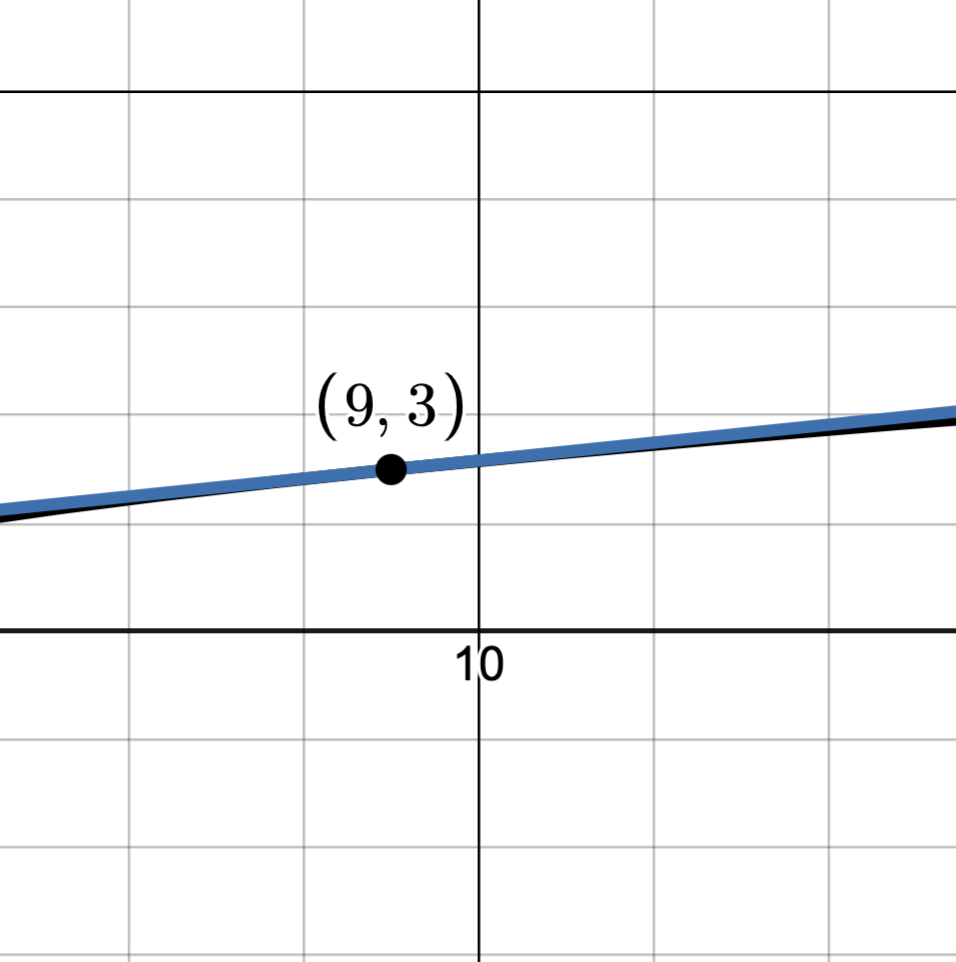
\includegraphics[width=2in]{./IntroductiontoDerivativesGraphics/TLEx203.png} 
 
 $y =r(t)$ and   $y = \frac{1}{6} \, t + \frac{3}{2}$  near $(9,3)$  

 \end{center}

\item As one might expect, we use this same strategy of rationalizing numerators to simplify the difference quotient to find $r'(t)$:

\[ \begin{array}{rcll}  

\dfrac{r(t+h) - r(t)}{h} & = & \dfrac{\sqrt{t+h} - \sqrt{t}}{h} & \\ [15pt]
												
												 & = & \dfrac{\left(\sqrt{t+h} - \sqrt{t}\right)}{h} \cdot \dfrac{\left(\sqrt{t+h} + \sqrt{t}\right)}{\left(\sqrt{t+h} + \sqrt{t}\right)} & \text{Multiply by the conjugate.} \\ [15pt]
										
												 & = &  \dfrac{\left(\sqrt{t+h}\right)^2 - \left(\sqrt{t}\right)^2}{h\left(\sqrt{t+h} + \sqrt{t}\right)} & \text{Difference of Squares.}\\ [15pt]
												
												& = &  \dfrac{(t+h) - t}{h\left(\sqrt{t+h} + \sqrt{t}\right)} & \\ [15pt]
												
												 & = &  \dfrac{h}{h\left(\sqrt{t+h} + \sqrt{t}\right)} & \\ [15pt]
												 
												 												 & = &  \dfrac{\cancelto{1}{h}}{\cancel{h}\left(\sqrt{t+h} + \sqrt{t}\right)} & \\ [15pt]
										
										
												 & = &  \dfrac{1}{\sqrt{t+h} + \sqrt{t}} & \\ 
												\end{array}\]	


We get \[r'(t) =  \lim_{h \rightarrow 0} \frac{1}{\sqrt{t+h} + \sqrt{t}} = \frac{1}{\sqrt{t+0} + \sqrt{t}}  = \frac{1}{2 \sqrt{t}}.\]   We check $r'(9) = \frac{1}{2\sqrt{9}} = \frac{1}{2(3)} = \frac{1}{6}$ as above.  \hfill \qed

\end{enumerate}

\end{enumerate}

\end{ex}




\newpage


\subsection{Exercises}

\label{ExercisesforAppDerivatives}
In Exercises \ref{diffquotexerfirsta} - \ref{diffquotexerlasta}, find the limit of the following difference quotients.

\begin{multicols}{2}

\begin{itemize}

\item  $\ds{\lim_{h \rightarrow 0} \dfrac{f(2+h) - f(2)}{h}}$

\item  $\ds{\lim_{h \rightarrow 0} \dfrac{f(x+h) - f(x)}{h}}$

\end{itemize}

\end{multicols}


\begin{multicols}{2}

\begin{enumerate}


\item $f(x) = 2x - 5$ \label{diffquotexerfirsta}
\item $f(x) = -3x + 5$

\setcounter{HW}{\value{enumi}}
\end{enumerate}
\end{multicols}

\begin{multicols}{2}
\begin{enumerate}
\setcounter{enumi}{\value{HW}}

\item $f(x) = 6$
\item $f(x) = 3x^2 - x$

\setcounter{HW}{\value{enumi}}
\end{enumerate}
\end{multicols}

\begin{multicols}{2}
\begin{enumerate}
\setcounter{enumi}{\value{HW}}

\item $f(x) = -x^2 + 2x - 1$
\item\label{diffquotexerlasta}  $f(x) = 4x^2$ 

\setcounter{HW}{\value{enumi}}
\end{enumerate}
\end{multicols}


In Exercises \ref{tangentlinepolyfirst} - \ref{tangentlinepolylast}, find:


\begin{itemize}

\item  $f'(2)  = \ds{\lim_{h \rightarrow 0} \dfrac{f(2+h) - f(2)}{h}}$

\item  The equation of the tangent line at $(2, f(2))$.  Check your answer graphically.

\item  $f'(x) = \ds{\lim_{h \rightarrow 0} \dfrac{f(x+h) - f(x)}{h}}$

\item  The equation of the tangent line at $(0,f(0))$.  Check your answer graphically.
 
\end{itemize}



\begin{multicols}{2}
\begin{enumerate}
\setcounter{enumi}{\value{HW}}

\item\label{tangentlinepolyfirst}  $f(x) = x-x^2$ 
\item\label{tangentlinepolylast} $f(x) = x^{3} + 1$

\setcounter{HW}{\value{enumi}}
\end{enumerate}
\end{multicols}




\begin{enumerate}
\setcounter{enumi}{\value{HW}}

\item  Find $f'(x) = \ds{\lim_{h \rightarrow 0} \dfrac{f(x+h) - f(x)}{h}}$  for $f(x) = mx + b\;$ where $m \neq 0$

\item\label{quadraticderivativeformulaexercise} \begin{enumerate}  \item Find $f'(x) = \ds{\lim_{h \rightarrow 0} \dfrac{f(x+h) - f(x)}{h}}$   for  $f(x) = ax^{2} + bx + c\;$ where $a \neq 0$.

\item  Solve $f'(x) = 0$ for $x$.  Does this look familiar?  Explain.

\end{enumerate}

\setcounter{HW}{\value{enumi}}
\end{enumerate}





In Exercises \ref{diffquotexerfirstb} - \ref{diffquotexerlastb}, find the limit of the following difference quotients:

\begin{multicols}{2}

\begin{itemize}

\item  $\ds{\lim_{\Delta x \rightarrow 0} \dfrac{f(-1+\Delta x) - f(-1)}{\Delta x}}$

\item  $\ds{\lim_{\Delta x \rightarrow 0} \dfrac{f(x+\Delta x) - f(x)}{\Delta x}}$

\end{itemize}

\end{multicols}

\begin{multicols}{2}
\begin{enumerate}
\setcounter{enumi}{\value{HW}}

\item $f(x) = \dfrac{2}{x}$  \label{diffquotexerfirstb}
\item $f(x) = \dfrac{3}{1-x}$

\setcounter{HW}{\value{enumi}}
\end{enumerate}
\end{multicols}

\begin{multicols}{2}
\begin{enumerate}
\setcounter{enumi}{\value{HW}}

\item  $f(x) = \dfrac{1}{x^2}$
\item\label{diffquotexerlastb}  $f(x) = \dfrac{2}{x+5}$

\setcounter{HW}{\value{enumi}}
\end{enumerate}
\end{multicols}

In Exercises \ref{rationaltangentfirst} - \ref{rationaltangentlast}, find the limit of the following:



\begin{itemize}

\item  $f'(-1) = \ds{\lim_{\Delta x \rightarrow 0} \dfrac{f(-1+\Delta x) - f(-1)}{\Delta x}}$

\item The equation of the tangent line at $(-1, f(-1))$.

\item  $f'(x) = \ds{\lim_{\Delta x \rightarrow 0} \dfrac{f(x+\Delta x) - f(x)}{\Delta x}}$

\item  The equation of the tangent line at $(0,f(0))$.

\end{itemize}

\begin{multicols}{2}
\begin{enumerate}

\setcounter{enumi}{\value{HW}}

\item\label{rationaltangentfirst} $f(x) = \dfrac{1}{4x-3}$ 
\item $f(x) = \dfrac{3x}{x+2}$ 

\setcounter{HW}{\value{enumi}}
\end{enumerate}
\end{multicols}

\begin{multicols}{2}
\begin{enumerate}
\setcounter{enumi}{\value{HW}}

\item $f(x) = \dfrac{x}{x - 9}$
\item\label{rationaltangentlast} $f(x) = \dfrac{x^2}{2x+1}$ 

\setcounter{HW}{\value{enumi}}
\end{enumerate}
\end{multicols}

In Exercises \ref{diffquotexerfirstc} - \ref{diffquotexerlastc},  find the limit of the following difference quotients:

\begin{multicols}{2}

\begin{itemize}

\item  $\ds{\lim_{\Delta t \rightarrow 0} \dfrac{g(\Delta t) - g(0)}{\Delta t}}$

\item  $\ds{\lim_{\Delta t \rightarrow 0} \dfrac{g(t+\Delta t) - g(t)}{\Delta t}}$

\end{itemize}

\end{multicols}


\begin{multicols}{2}
\begin{enumerate}
\setcounter{enumi}{\value{HW}}

\item  $g(t) = \sqrt{9-t}$  \label{diffquotexerfirstc}
\item  $g(t) = \sqrt{2t+1}$   \label{diffquotexerlastc}


\setcounter{HW}{\value{enumi}}
\end{enumerate}
\end{multicols}

In Exercises \ref{tangentrootfirst} - \ref{tangentrootlast},  find the following:



\begin{itemize}

\item  $g'(0) = \ds{\lim_{\Delta t \rightarrow 0} \dfrac{g(\Delta t) - g(0)}{\Delta t}}$

\item  The equation of the tangent line at $(0, g(0))$.

\item  $g'(t) =  \ds{\lim_{\Delta t \rightarrow 0} \dfrac{g(t+\Delta t) - g(t)}{\Delta t}}$

\item  The equation of the tangent line at $(1, g(1))$.

\end{itemize}




\begin{multicols}{2}
\begin{enumerate}
\setcounter{enumi}{\value{HW}}

\item\label{tangentrootfirst}  $g(t) = \sqrt{-4t+5}$
\item  \label{tangentrootlast} $g(t) = \sqrt{4-t}$


\setcounter{HW}{\value{enumi}}
\end{enumerate}
\end{multicols}



\begin{enumerate}
\setcounter{enumi}{\value{HW}}

\item  For  $g(t) = t \sqrt{t}$:

\begin{enumerate}

\item  Explain why $g'(0) = \ds{\lim_{\Delta t \rightarrow 0} \dfrac{g(\Delta t) - g(0)}{\Delta t}}$ does not exist.

\item Find the \index{derivative from the right}\index{derivative ! from the right} derivative \textbf{from the right} at $t=0$:  $g_{+}'(0) = \ds{\lim_{\Delta t \rightarrow 0^{+}} \dfrac{g(\Delta t) - g(0)}{\Delta t}}$

\item  Find $y = g_{+}'(0) (x-0) + g(0)$ and interpret.

\item Find  $g'(t) =  \ds{\lim_{\Delta t \rightarrow 0} \dfrac{g(t+\Delta t) - g(t)}{\Delta t}}$.  Assume $t>0$.

\end{enumerate}


\item  \begin{enumerate} \item Find  $g'(t) =  \ds{\lim_{\Delta t \rightarrow 0} \dfrac{g(t+\Delta t) - g(t)}{\Delta t}}$ for  $g(t) = \sqrt{at+b}$, $a \neq 0$. 

\smallskip

\item What restrictions do you place on $t$ so your formula is valid?

\end{enumerate}


\setcounter{HW}{\value{enumi}}
\end{enumerate}


\begin{enumerate}
\setcounter{enumi}{\value{HW}}

\item Let  $f(x) =|x|$.  

\begin{enumerate}

\item  Explain why $f$ is continuous at $x = 0$.

\item\label{cornerex} Show $f'(0)$ does not exist by showing $\ds{\lim_{h \rightarrow 0^{-}} \dfrac{f(h) - f(0)}{h} =-1}$ but  $\ds{\lim_{h \rightarrow 0^{+}} \dfrac{f(h) - f(0)}{h} = 1}$.  

\smallskip
        
\item  Graph $y = f(x)$ near $(0,0)$.  Interpret your answer to number \ref{cornerex} graphically.

\smallskip

\item  Find and simplify  $f'(x) =  \ds{\lim_{h \rightarrow 0} \dfrac{|x+h| - |x|}{h}}$ assuming $x \neq 0$.

\smallskip

\textbf{HINT:}  Consider the two cases $x > 0$ and $x < 0$ \ldots
        
\smallskip

\end{enumerate}


\item Let  $g(t) = \sqrt[3]{t}$.  

\begin{enumerate}

\item Explain why $g$ is continuous at $t = 0$.

\item\label{verticaltangentex} Show $g'(0)$ does not exist by showing $\ds{\lim_{\Delta t \rightarrow 0} \dfrac{g(\Delta t) - g(0)}{\Delta t} = \infty}$.  

\smallskip
        
\item  Graph $y = g(t)$ near $(0,0)$.  Interpret your answer to number \ref{verticaltangentex} graphically.

\smallskip

\item  Find and simplify  $g'(t) =  \ds{\lim_{\Delta t \rightarrow 0} \dfrac{g(t+\Delta t) - g(t)}{\Delta t}}$ assuming $t \neq 0$.

\smallskip

\textbf{HINT:}  $(a-b)\left(a^2+ab+b^2\right) = a^3 - b^3$ 
        
\smallskip

\end{enumerate}

\item Let  $h(x) = x^{\frac{2}{3}}$.  

\begin{enumerate}

\item Explain why $h$ is continuous at $x = 0$.

\item\label{cuspex} Show $h'(0)$ does not exist by showing $\ds{\lim_{\Delta x \rightarrow 0^{-}} \dfrac{h(\Delta x) - h(0)}{\Delta x} = -\infty}$ and $\ds{\lim_{\Delta x \rightarrow 0^{+}} \dfrac{h(\Delta x) - h(0)}{\Delta x} = \infty}$

\smallskip
        
\item  Graph $y = h(x)$ near $(0,0)$.  Interpret your answer to number \ref{cuspex} graphically.

\smallskip

\item  Find and simplify  $h'(x) =  \ds{\lim_{\Delta x \rightarrow 0} \dfrac{h(x+\Delta x) - h(x)}{\Delta x}}$ assuming $x \neq 0$.

\smallskip

\textbf{HINT:}  $(a-b)\left(a^2+ab+b^2\right) = a^3 - b^3$ and $a^2 - b^2 = (a+b)(a-b)$.
        
\smallskip

\end{enumerate}

\item  Recall from Exercise \ref{JasonHammerExercise1} in Section \ref{QuadraticFunctions} that Carl's friend Jason participates in the Highland Games. In one event, the hammer throw, the height $h(t)$ in feet of the hammer above the ground $t$ seconds after Jason lets it go is modeled by the function $h(t) = -16t^2 +  22.08t + 6$. 

\begin{enumerate}

\item  Find and simplify a formula for the velocity of the hammer, $v(t) = h'(t) = \ds{\lim_{\Delta t \rightarrow 0} \dfrac{h(t + \Delta t) - h(t)}{\Delta t}}$.

\item  Find and interpret $v(0)$.

\item  Solve $v(t) = 0$ and interpret.

\item  Find the velocity of the hammer when it hits the ground, rounded to three decimal places.

\end{enumerate}

\item  In Exercise \ref{fueleconomyexercise}  in Section \ref{QuadraticFunctions}, the average fuel economy $F(t)$ in miles per gallon (mpg) for passenger cars in the US $t$ years after 1980 is modeled by  $F(t) = -0.0076t^2+0.45t + 16$, $0 \leq t \leq 28$. 

\begin{enumerate}

\item  Find and simplify a formula for  $F'(t) = \ds{\lim_{h \rightarrow 0} \dfrac{F(t + h) - F(t)}{h}}$.

\item\label{fueleconomytrendexercise}  Find and interpret $F'(0)$, $F'(5)$ and $F'(10)$.

\item  Interpret the trend you observe in your answers to part \ref{fueleconomytrendexercise}.

\end{enumerate}

\item\label{MarginalCostDerivativeExercise} Let us return to Example \ref{marginalsetupex} where  $C(x) = .03x^{3} - 4.5x^{2} + 225x + 250$ denotes the cost, in dollars,  of producing $x$ PortaBoy game systems.

\begin{enumerate}

\item  Find and interpret $C'(75) = \ds{\lim_{h \rightarrow 0} \dfrac{C(75+h) - C(75)}{h}}$.

\item  Recall in Exercise \ref{AverageCostMarginalCostExercise} in Section \ref{FunctionArithmetic}, we found the marginal cost, $MC(75) = 58.53$,   which means it will cost an additional $\$ 58.53$ to produce the $76$th item.  Compare $C'(75)$ and $MC(75)$. 

\end{enumerate}

\setcounter{HW}{\value{enumi}}
\end{enumerate}

\newpage


In Exercises \ref{MatchFcnDerivative1first} - \ref{MatchFcnDerivative1last}, match the graph of the function with a plausible graph of its derivative.

\begin{center}

\begin{multicols}{2}

\begin{enumerate}
\setcounter{enumi}{\value{HW}}

\item \label{MatchFcnDerivative1first}$y = f(x)$:

\setcounter{HW}{\value{enumi}}
\end{enumerate}

Graph A:

\end{multicols}


\begin{multicols}{2}

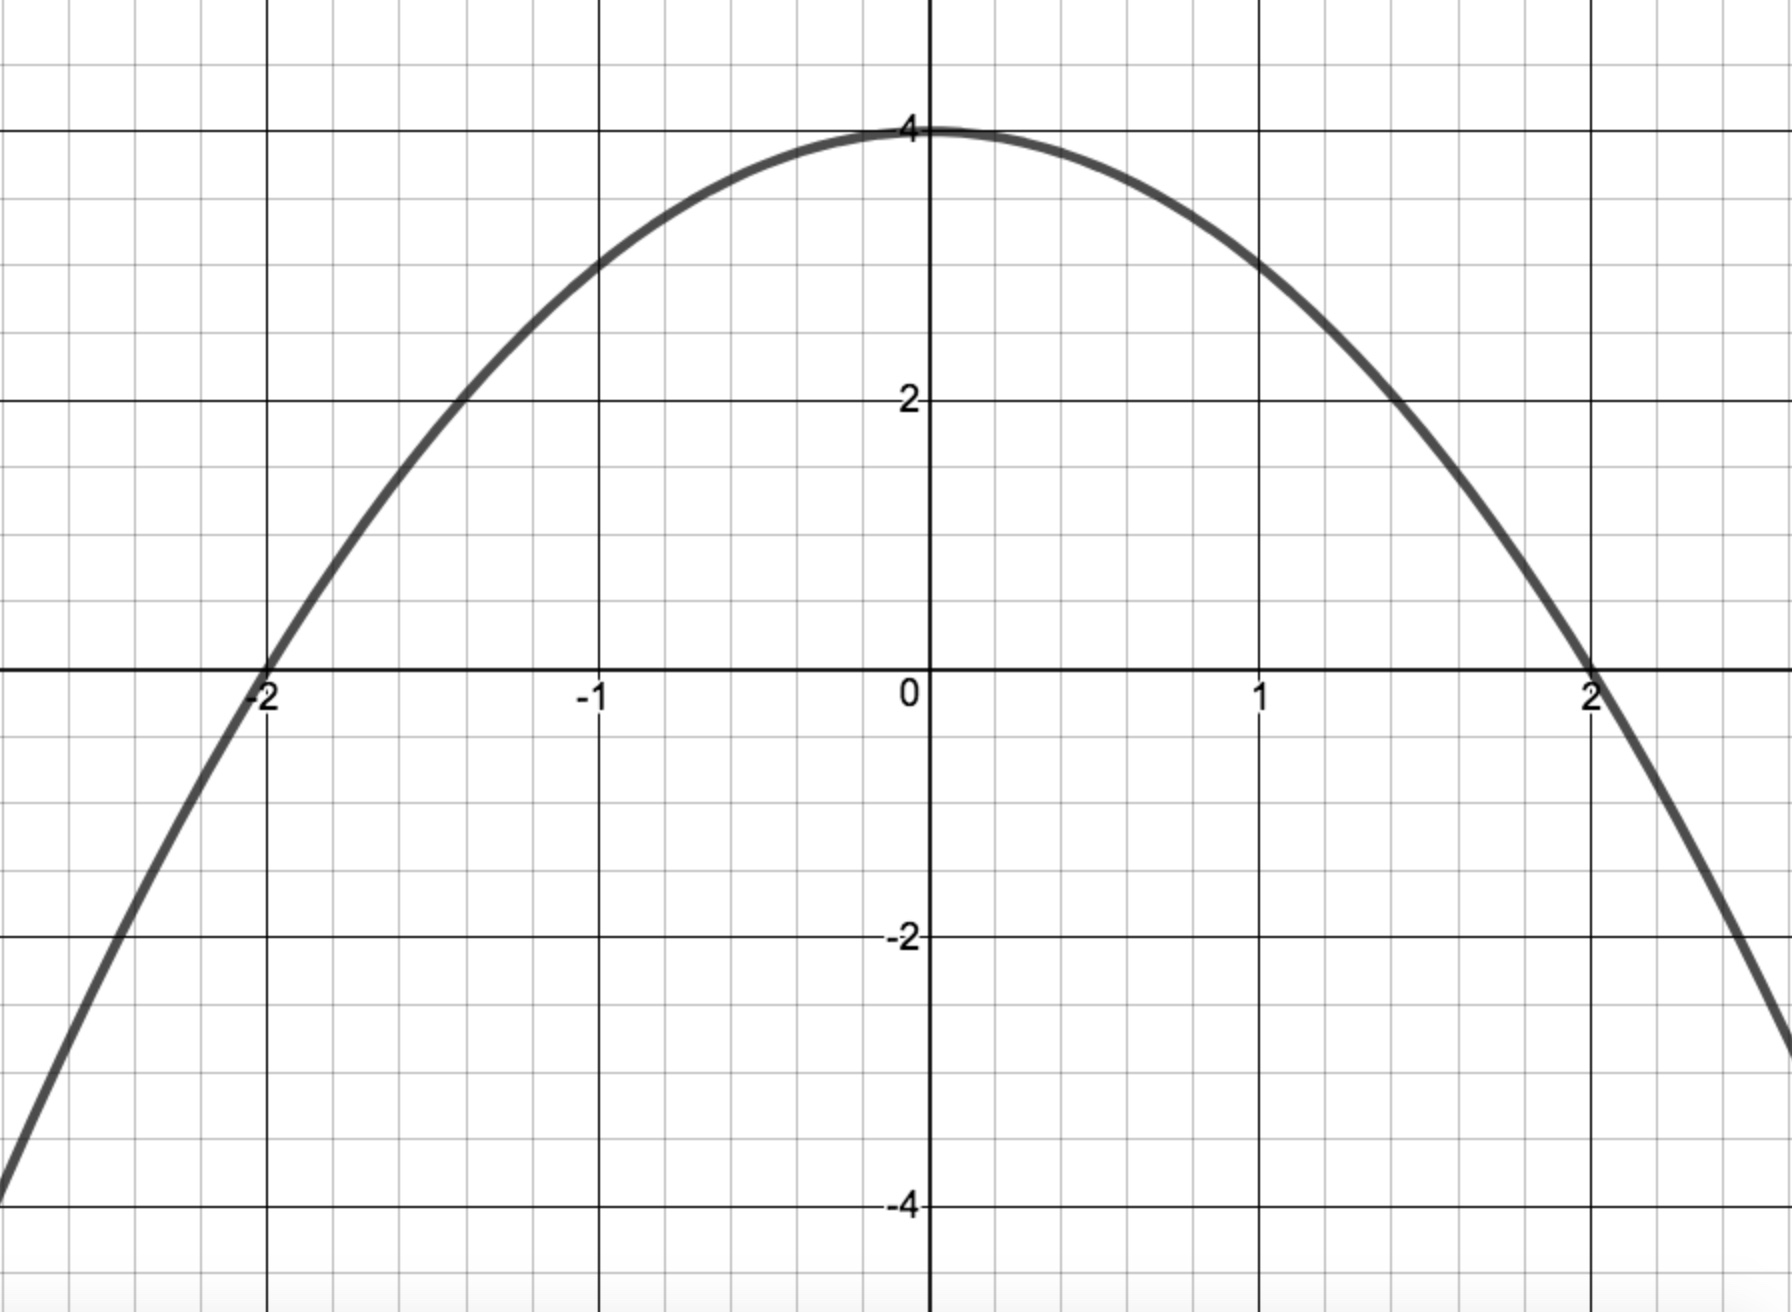
\includegraphics[width=2.75in]{./IntroductiontoDerivativesGraphics/MatchFunc01.jpeg}

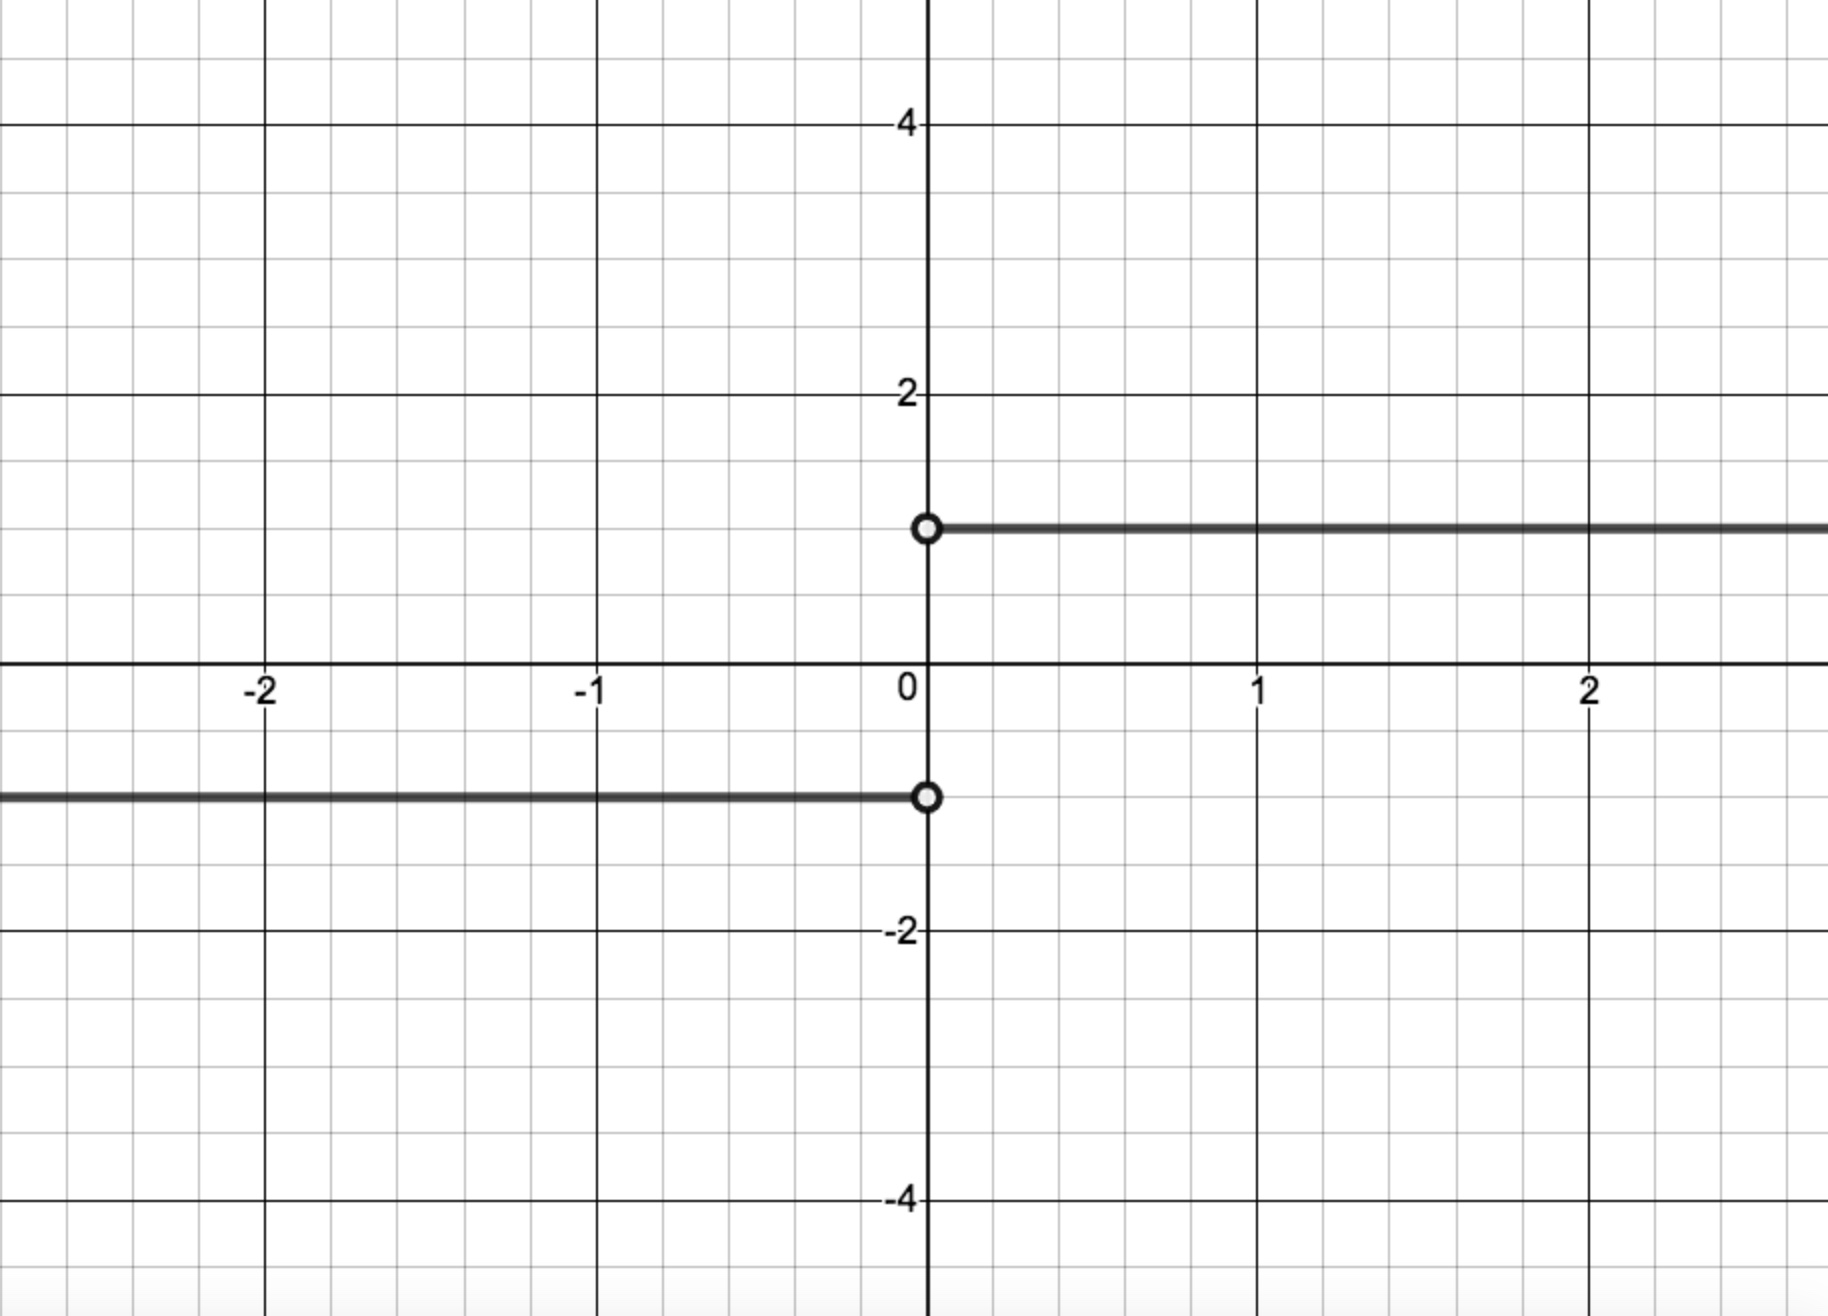
\includegraphics[width=2.75in]{./IntroductiontoDerivativesGraphics/MatchDeriv03.jpeg}

\end{multicols}



\begin{multicols}{2}

\begin{enumerate}
\setcounter{enumi}{\value{HW}}

\item $y = g(x)$:

\setcounter{HW}{\value{enumi}}
\end{enumerate}

Graph B:

\end{multicols}

\begin{multicols}{2}

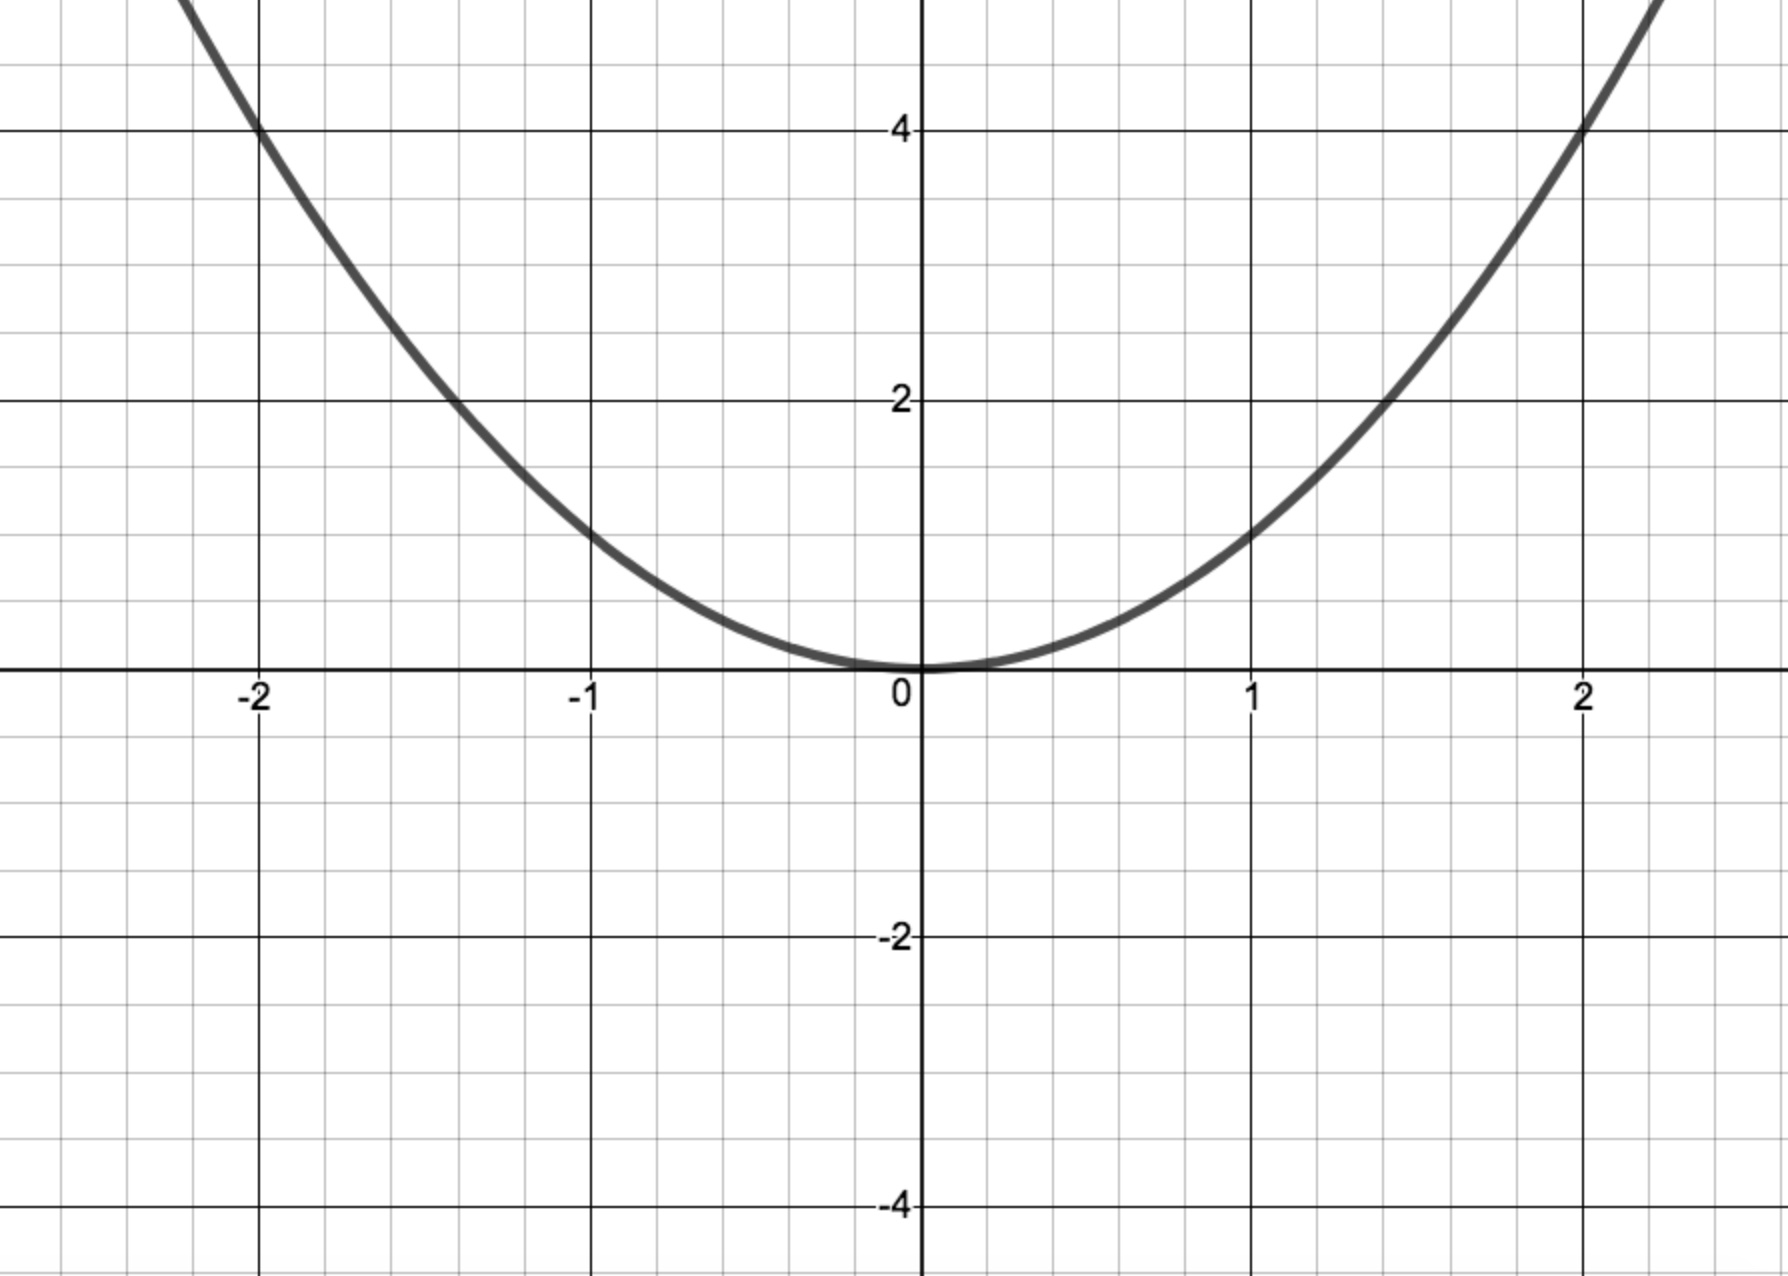
\includegraphics[width=2.75in]{./IntroductiontoDerivativesGraphics/MatchFunc02.jpeg}

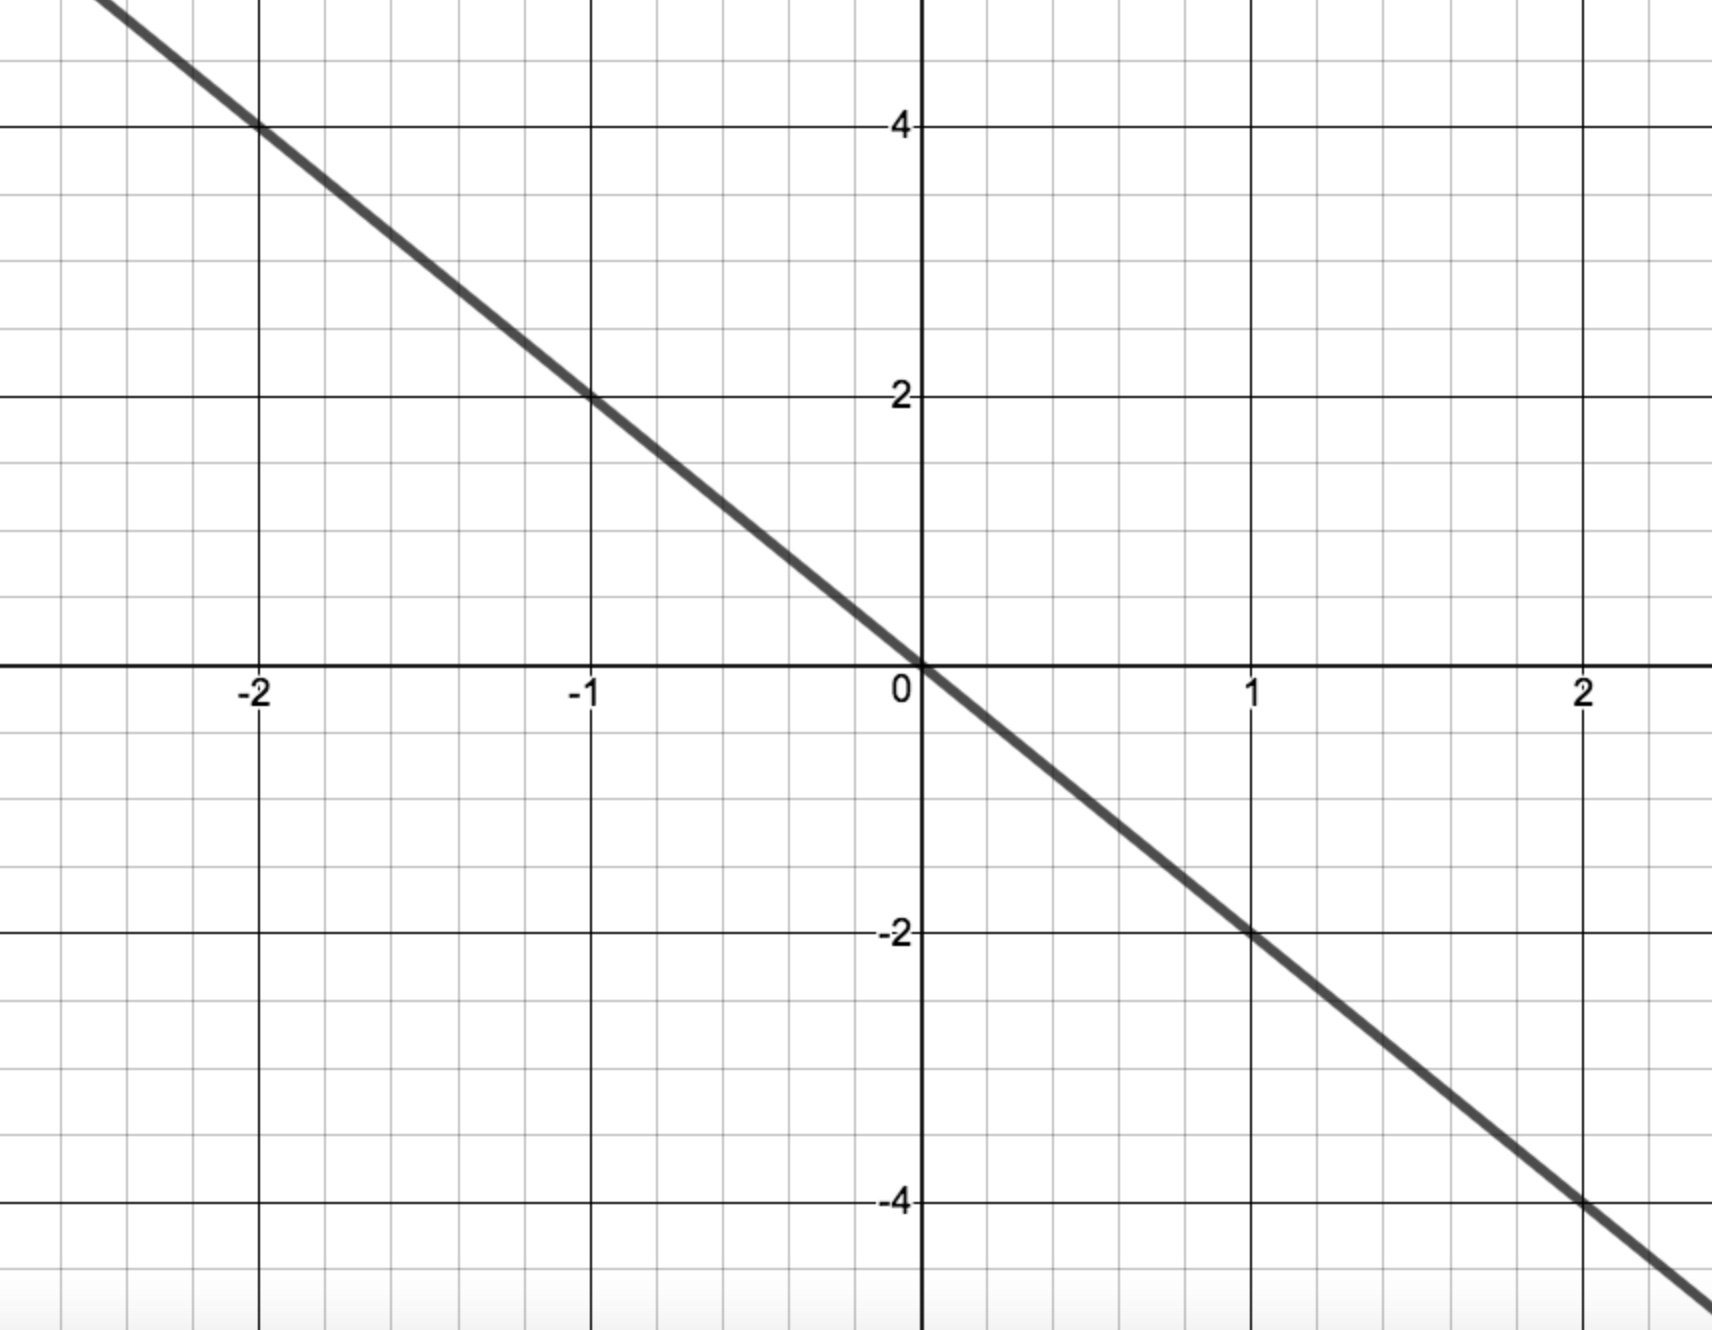
\includegraphics[width=2.75in]{./IntroductiontoDerivativesGraphics/MatchDeriv01.jpeg}

\end{multicols}


\begin{multicols}{2}

\begin{enumerate}
\setcounter{enumi}{\value{HW}}

\item \label{MatchFcnDerivative1last} $y = h(x)$:

\setcounter{HW}{\value{enumi}}
\end{enumerate}


Graph C:

\end{multicols}




\begin{multicols}{2}

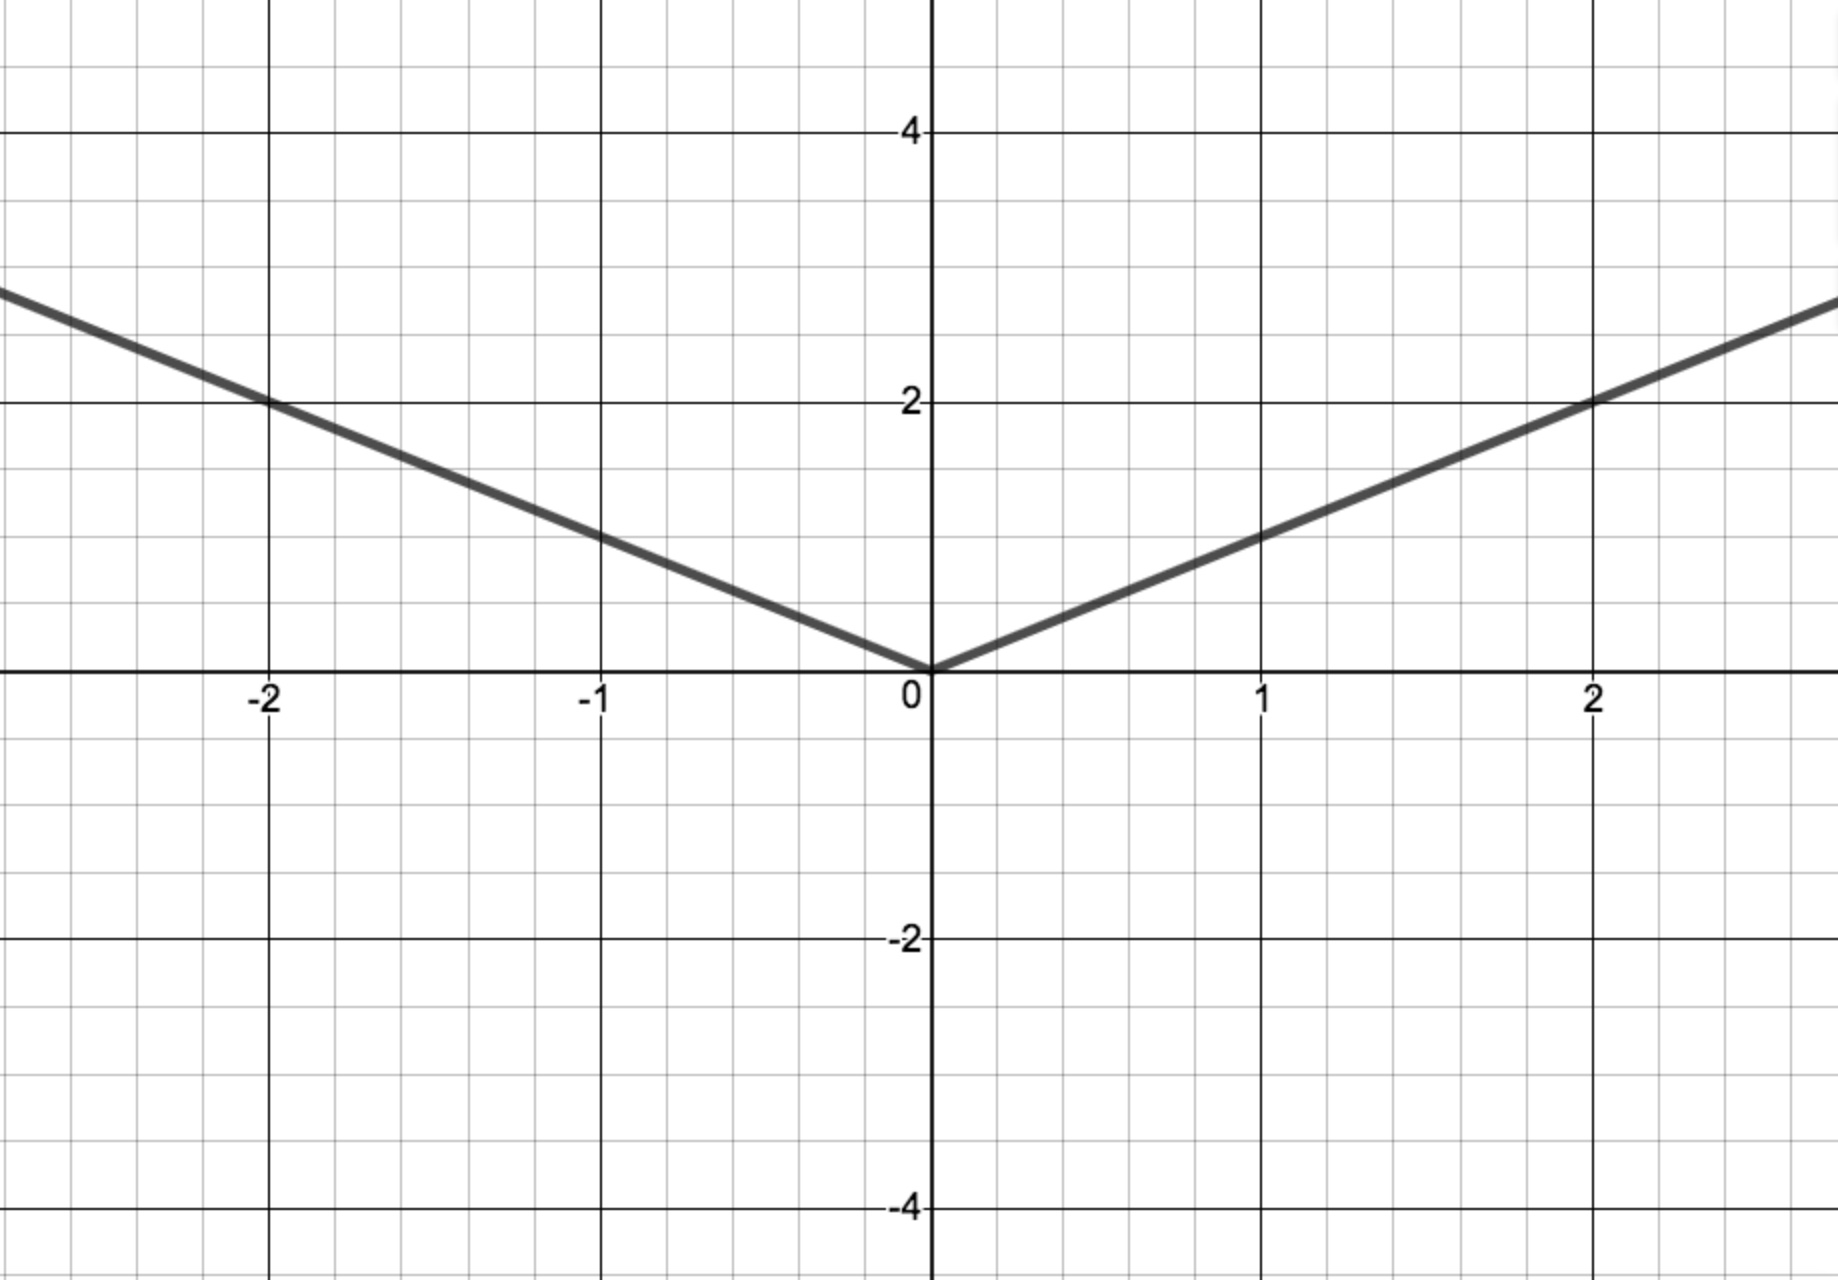
\includegraphics[width=2.75in]{./IntroductiontoDerivativesGraphics/MatchFunc03.jpeg}

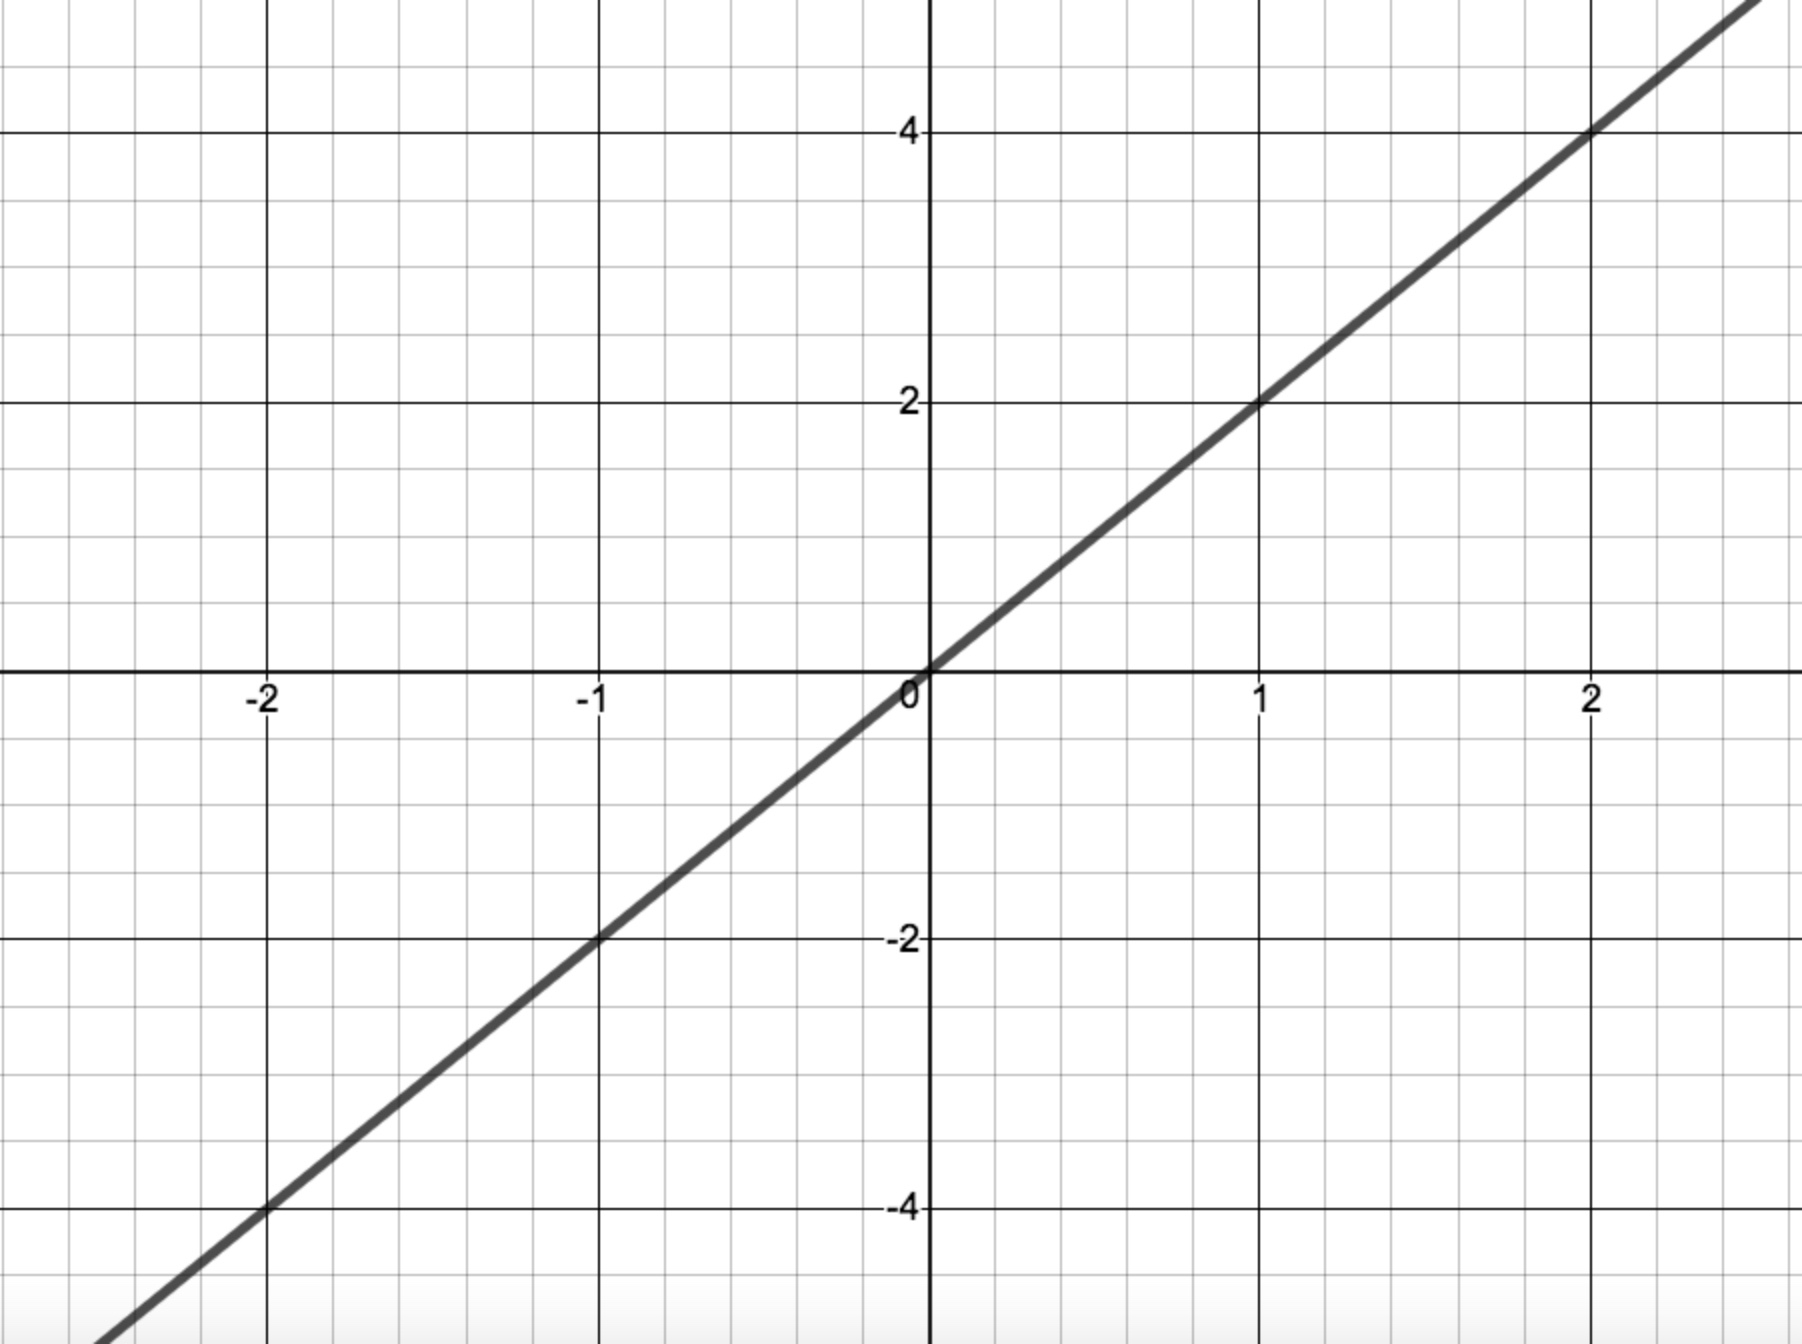
\includegraphics[width=2.75in]{./IntroductiontoDerivativesGraphics/MatchDeriv02.jpeg}

\end{multicols}


\end{center}

In Exercises \ref{MatchFcnDerivative2first} - \ref{MatchFcnDerivative2last}, match the graph of the function with a plausible graph of its derivative.


\begin{center}


\begin{multicols}{2}

\begin{enumerate}
\setcounter{enumi}{\value{HW}}

\item \label{MatchFcnDerivative2first} $y = f(x)$:

\setcounter{HW}{\value{enumi}}
\end{enumerate}

Graph A:

\end{multicols}




\begin{multicols}{2}

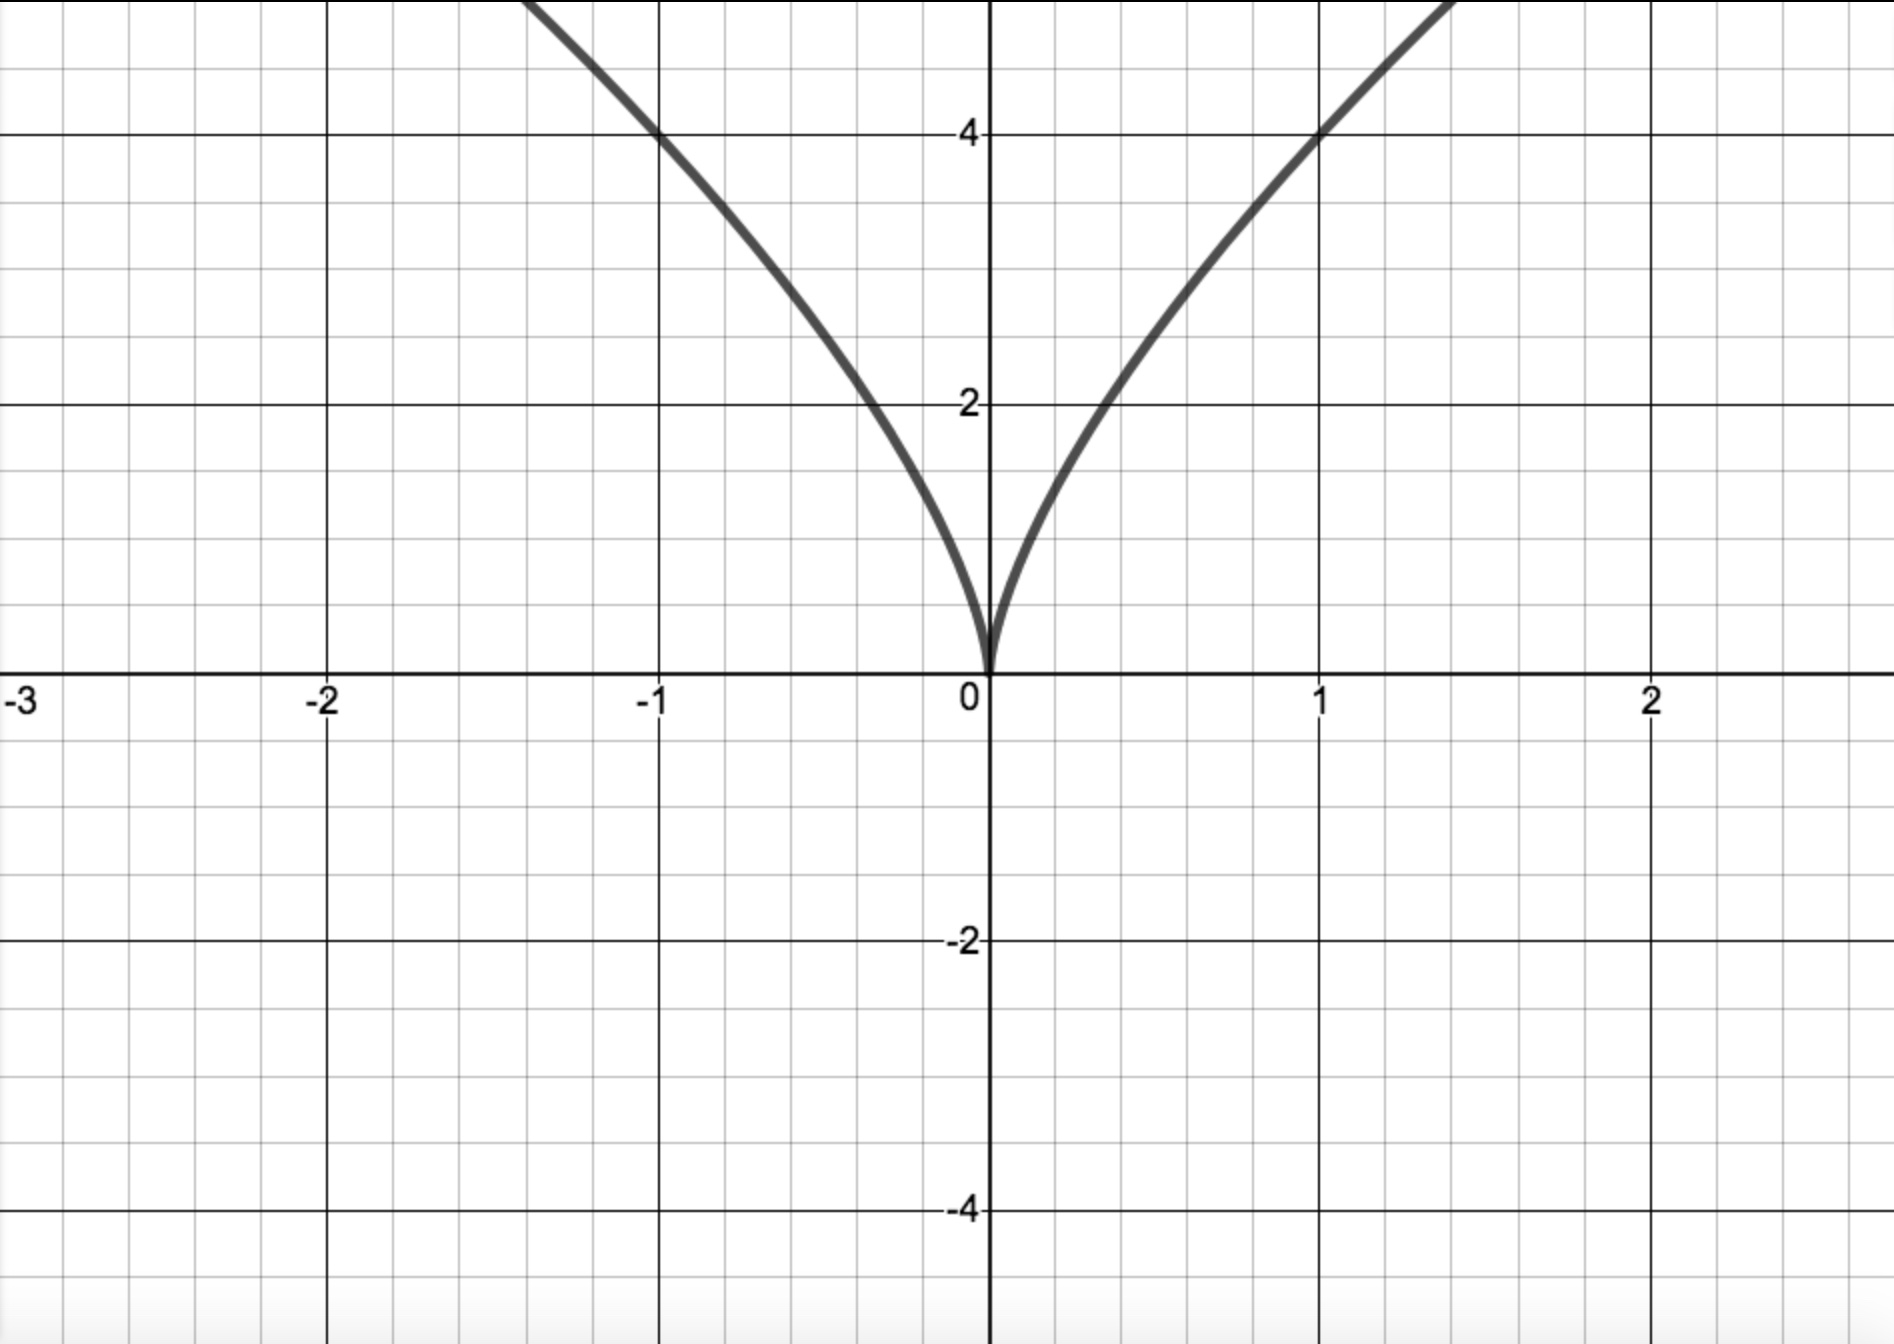
\includegraphics[width=2.75in]{./IntroductiontoDerivativesGraphics/MatchFunc04.jpeg}

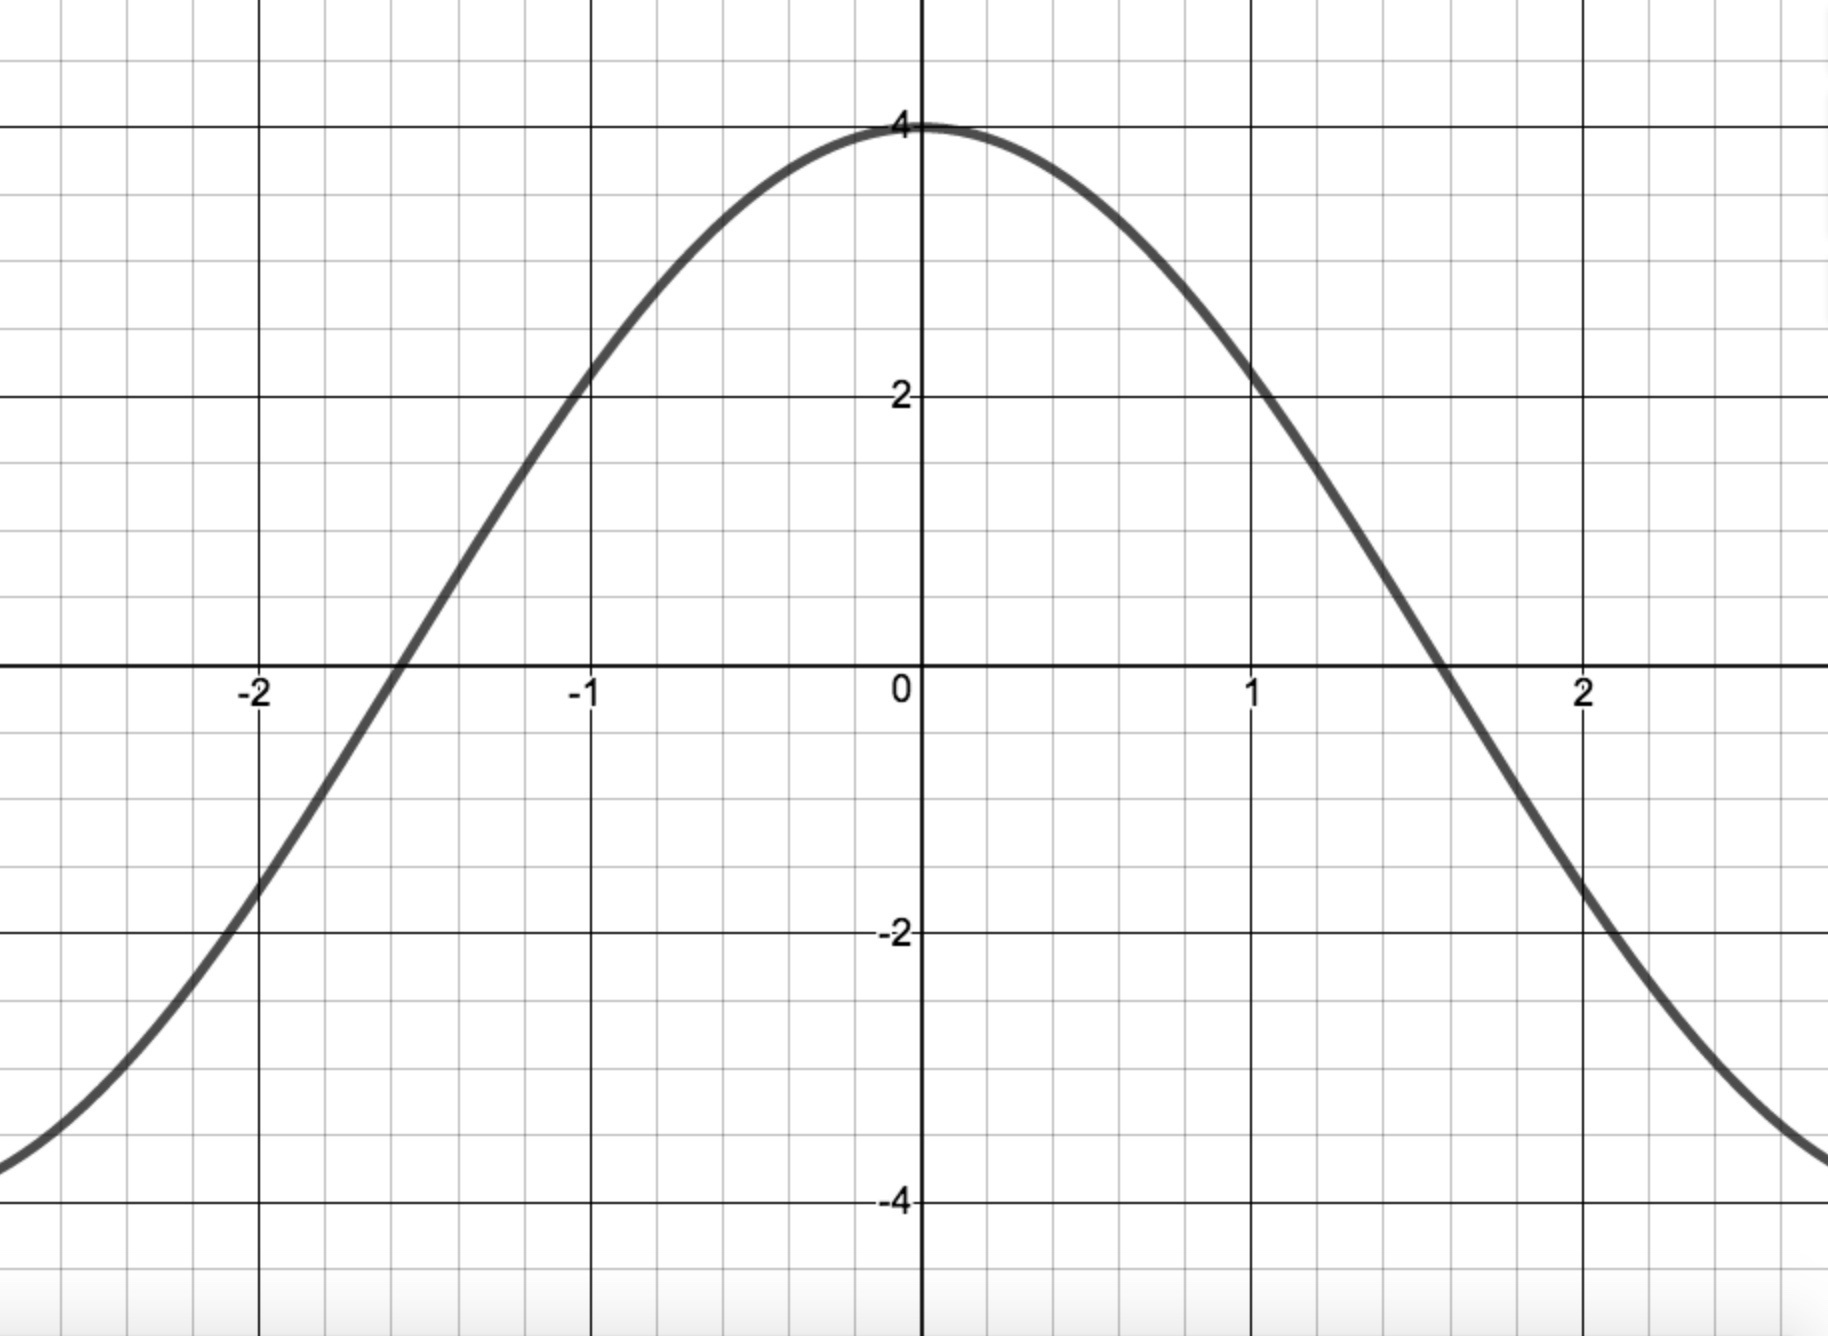
\includegraphics[width=2.75in]{./IntroductiontoDerivativesGraphics/MatchDeriv06.jpeg}

\end{multicols}



\begin{multicols}{2}

\begin{enumerate}
\setcounter{enumi}{\value{HW}}

\item $y = g(x)$:

\setcounter{HW}{\value{enumi}}
\end{enumerate}

Graph B:

\end{multicols}




\begin{multicols}{2}

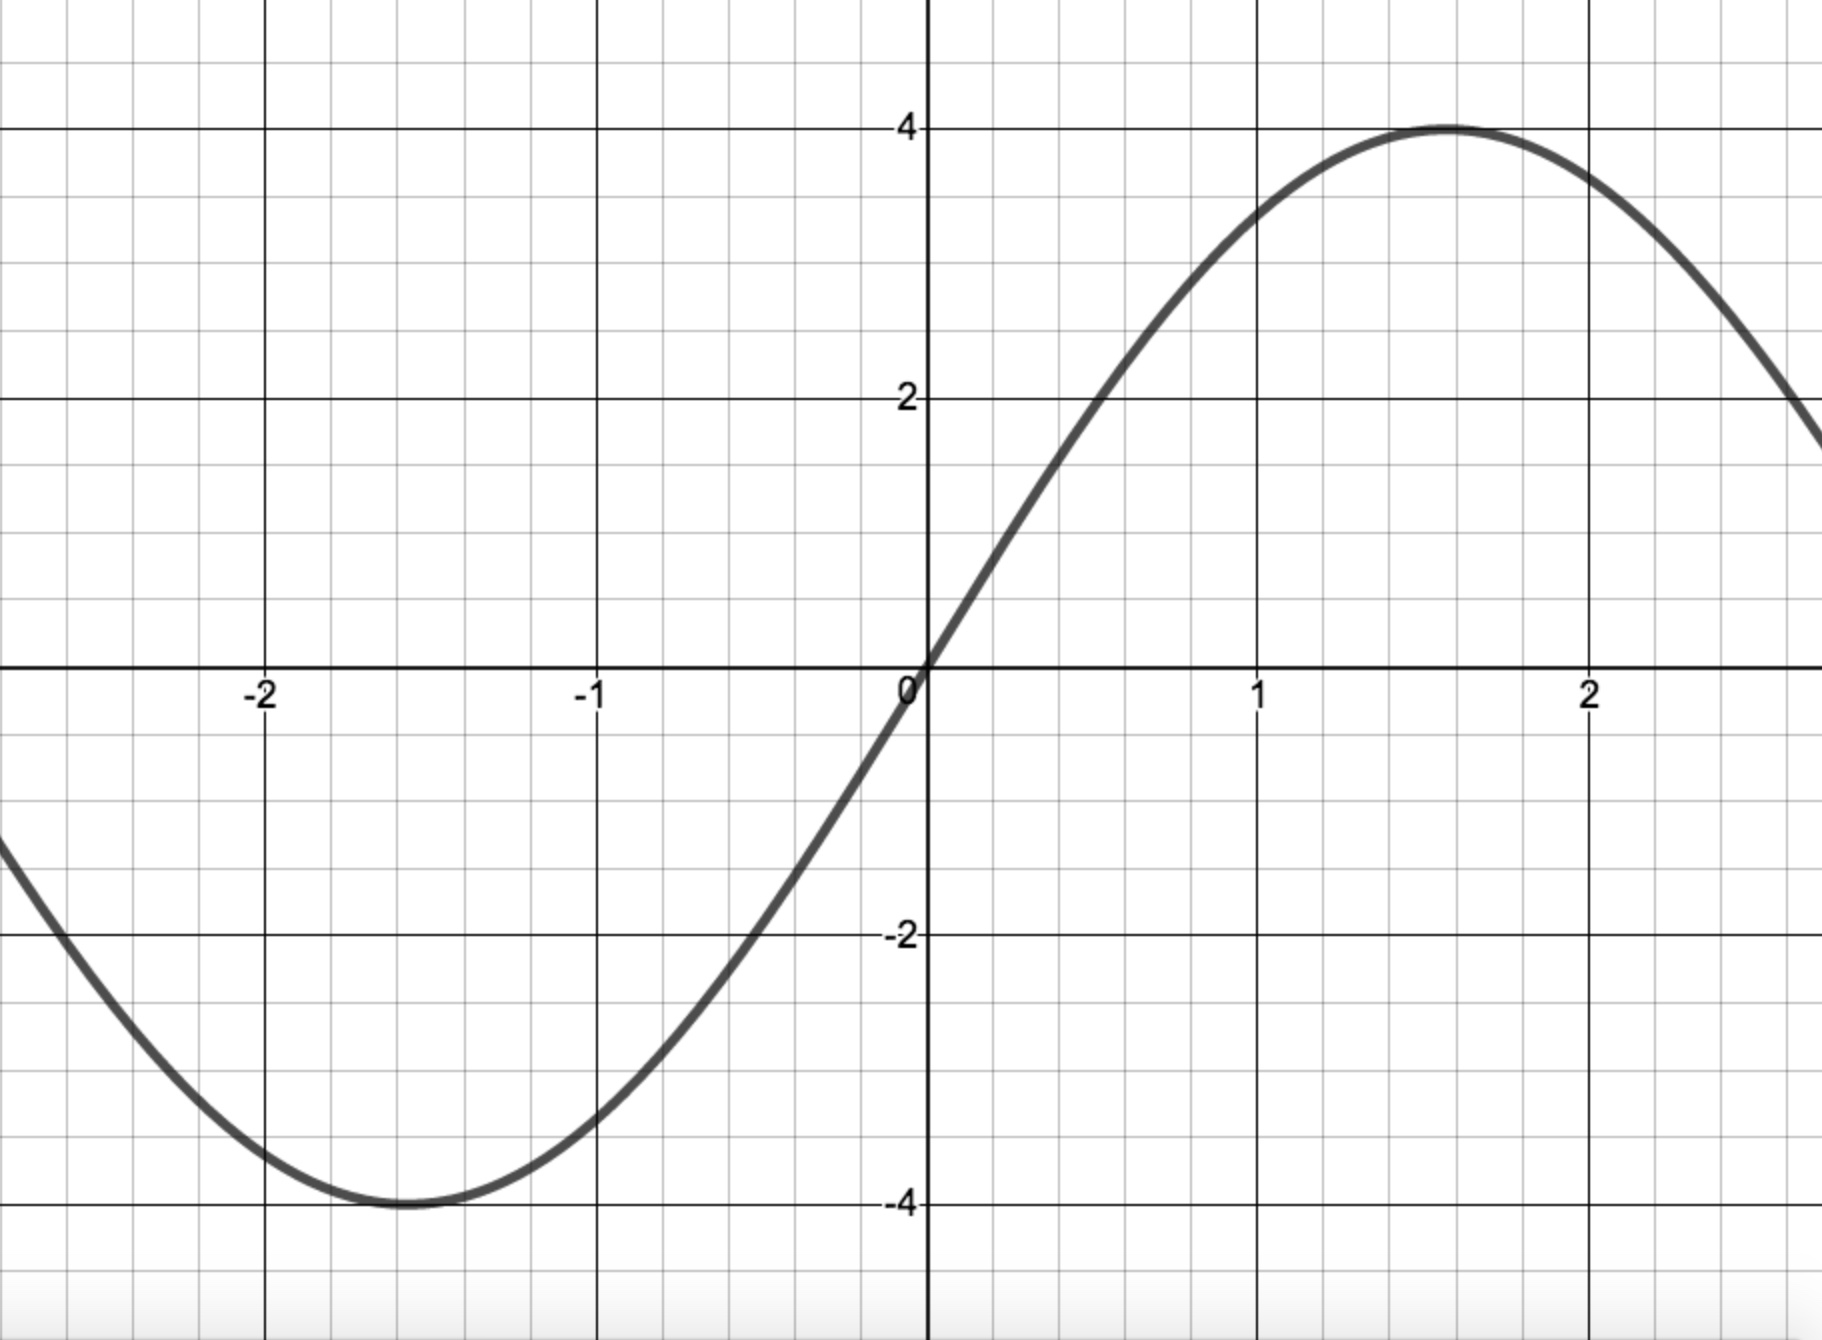
\includegraphics[width=2.75in]{./IntroductiontoDerivativesGraphics/MatchFunc06.jpeg}

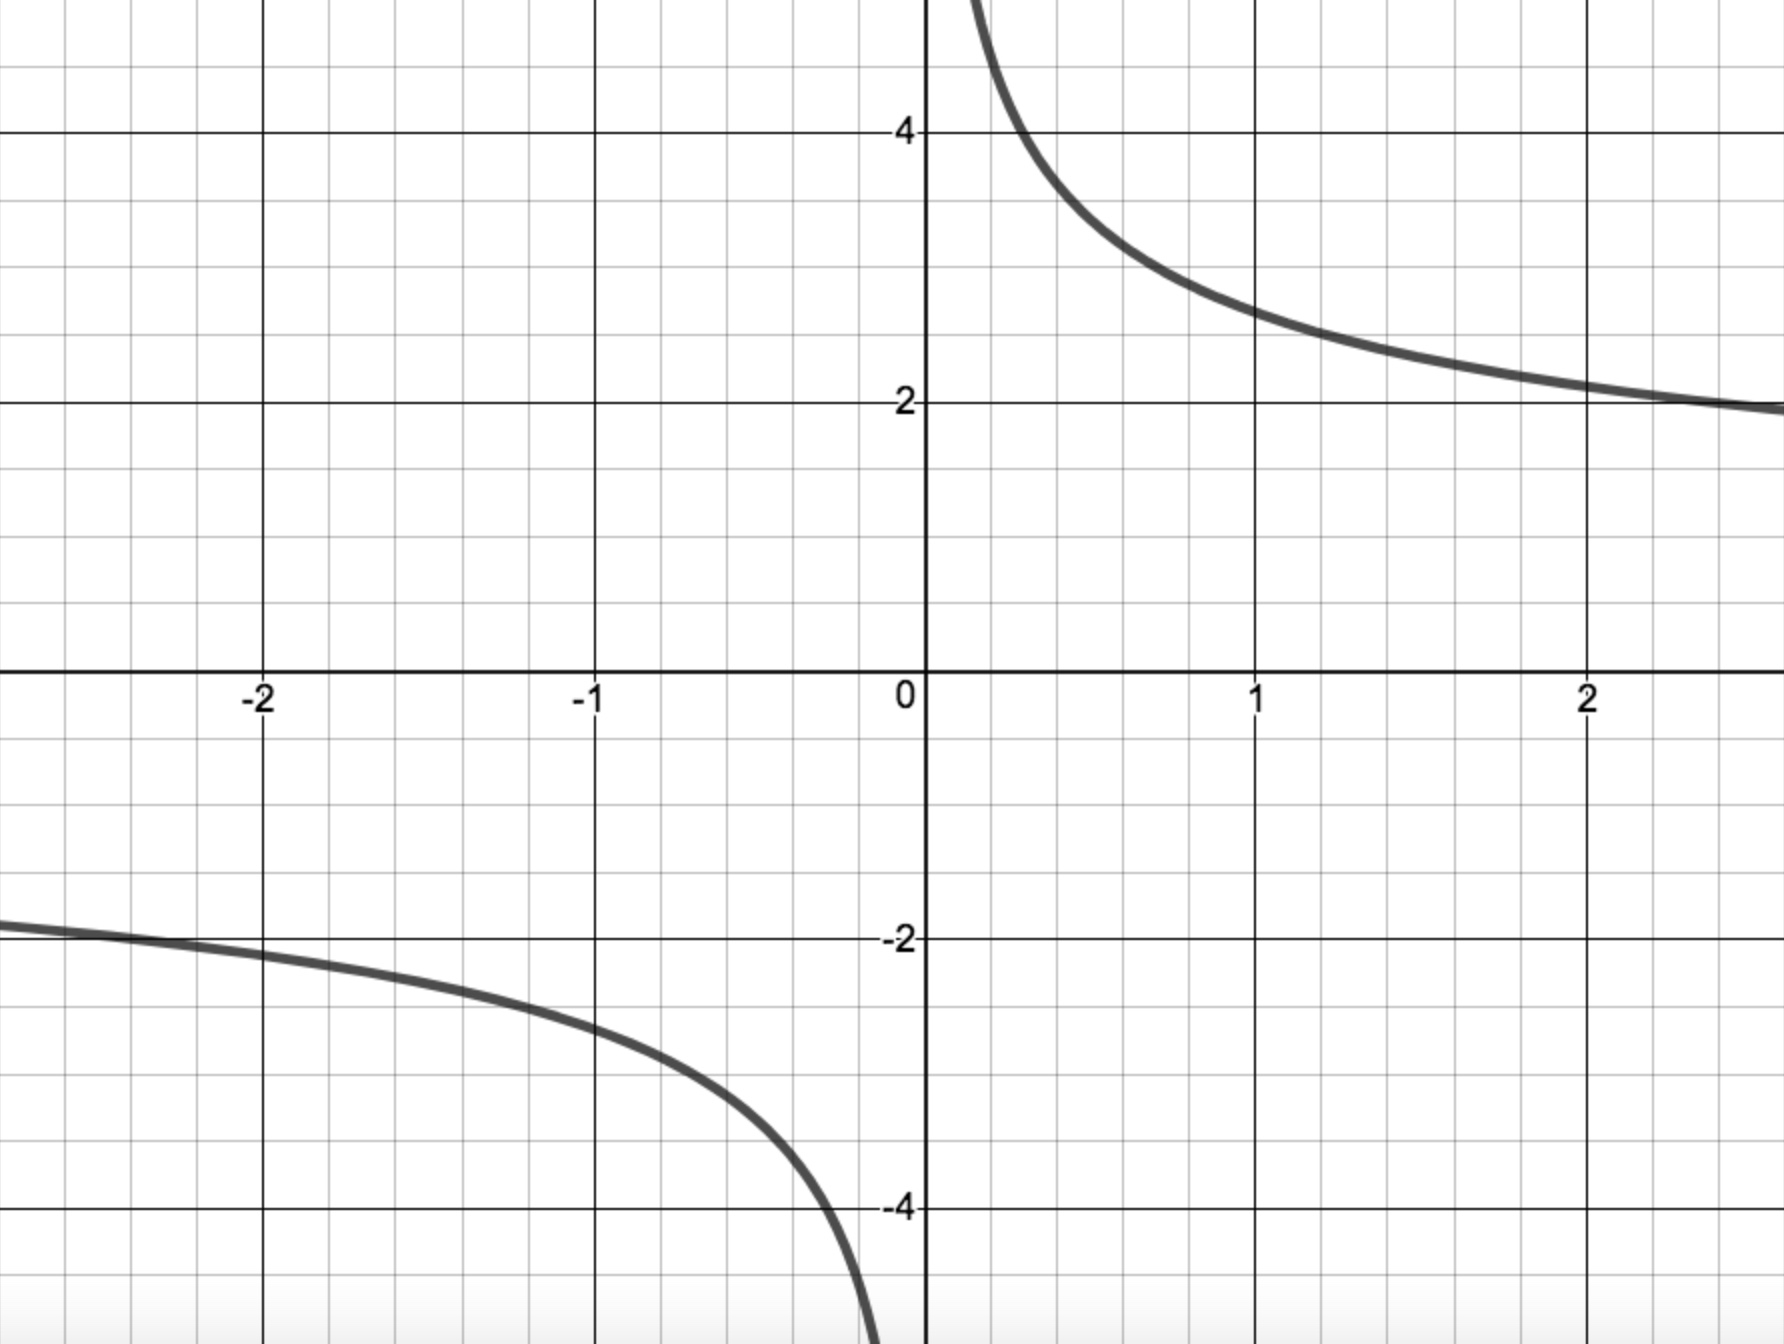
\includegraphics[width=2.75in]{./IntroductiontoDerivativesGraphics/MatchDeriv04.jpeg}

\end{multicols}



\begin{multicols}{2}

\begin{enumerate}
\setcounter{enumi}{\value{HW}}

\item \label{MatchFcnDerivative2last}  $y = h(x)$:

\setcounter{HW}{\value{enumi}}
\end{enumerate}

Graph C:

\end{multicols}



\begin{multicols}{2}

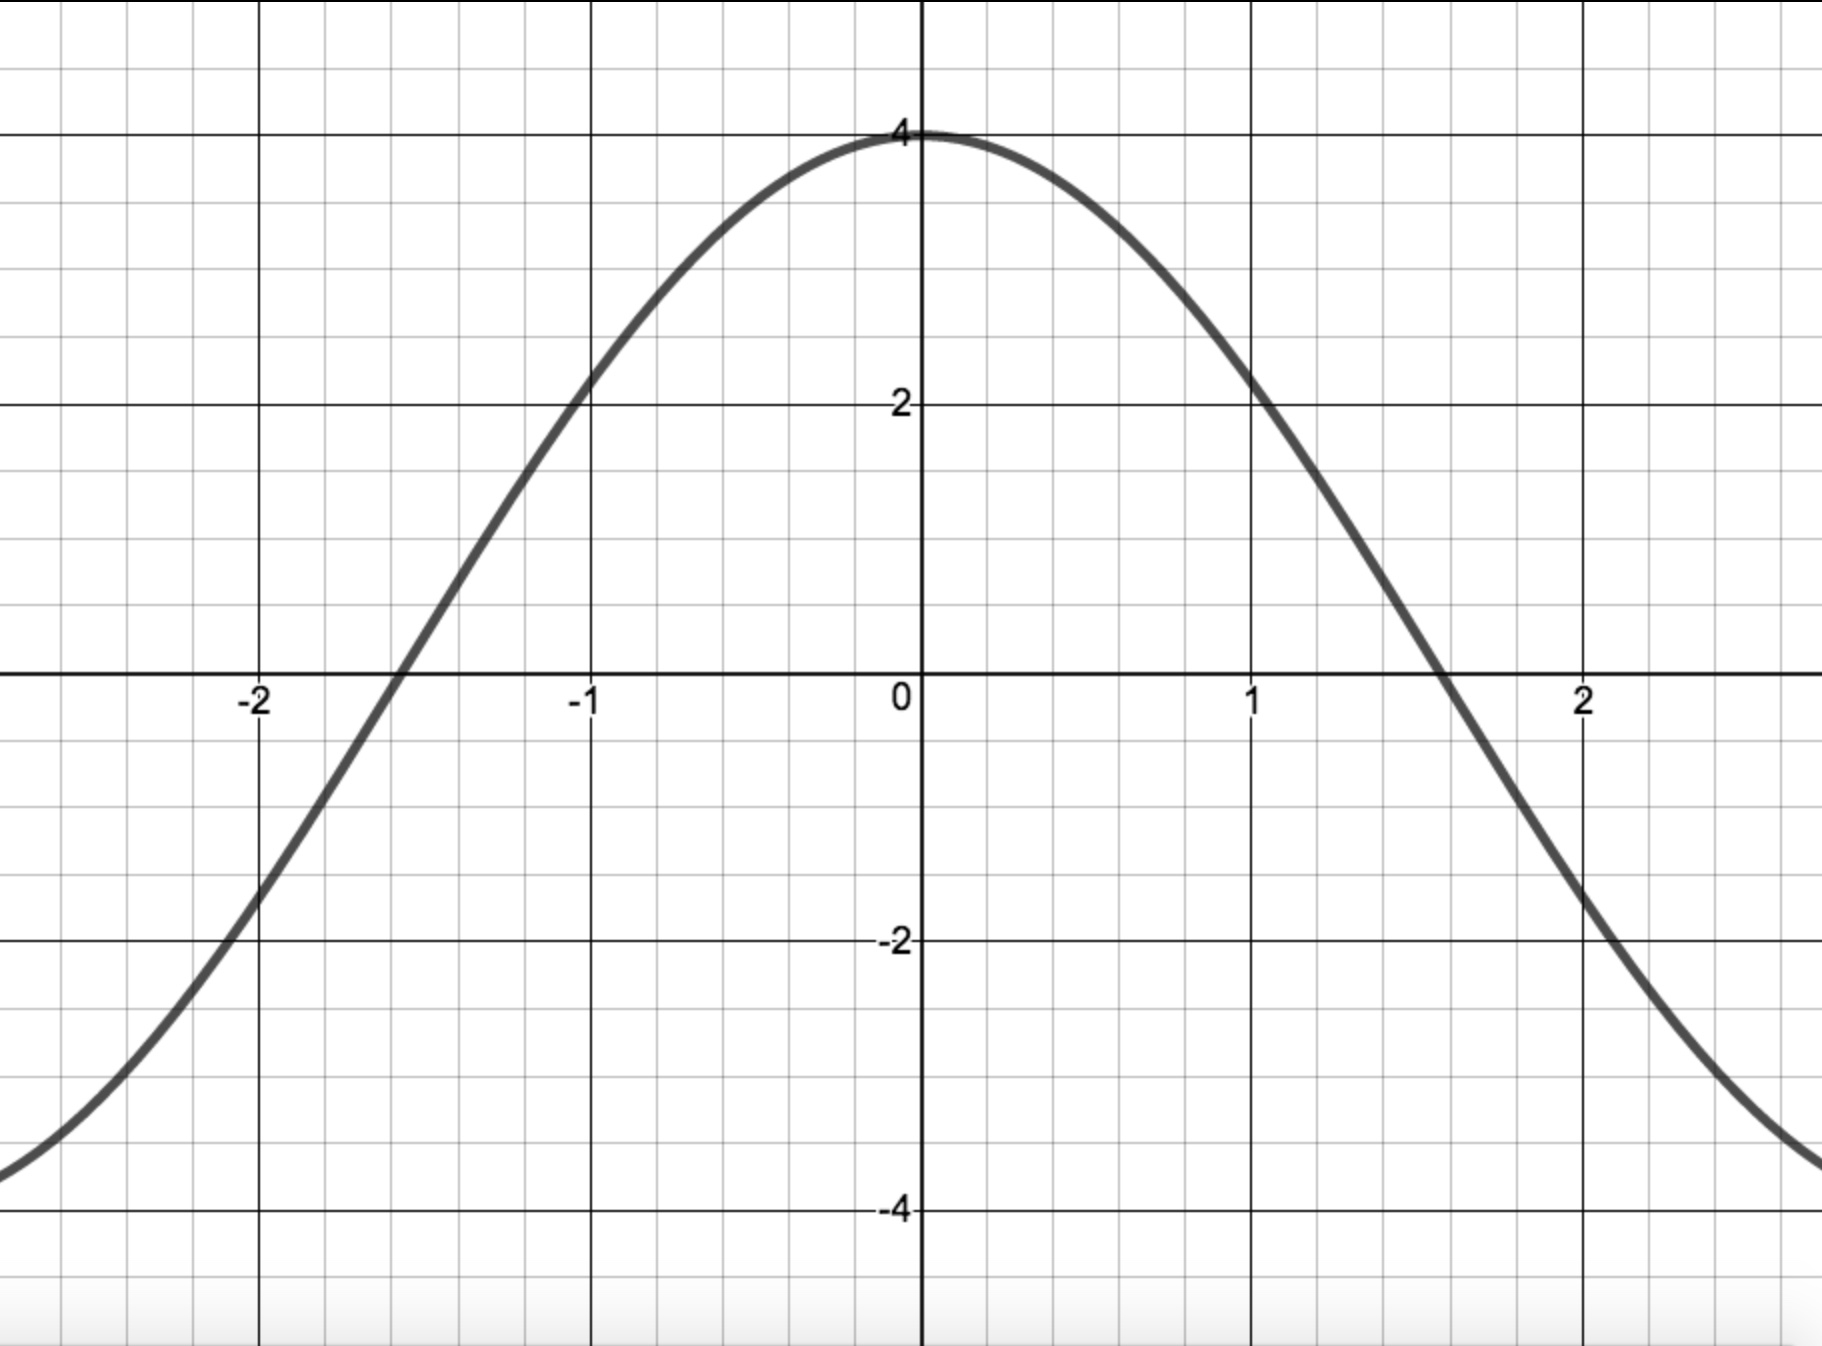
\includegraphics[width=2.75in]{./IntroductiontoDerivativesGraphics/MatchFunc05.jpeg}

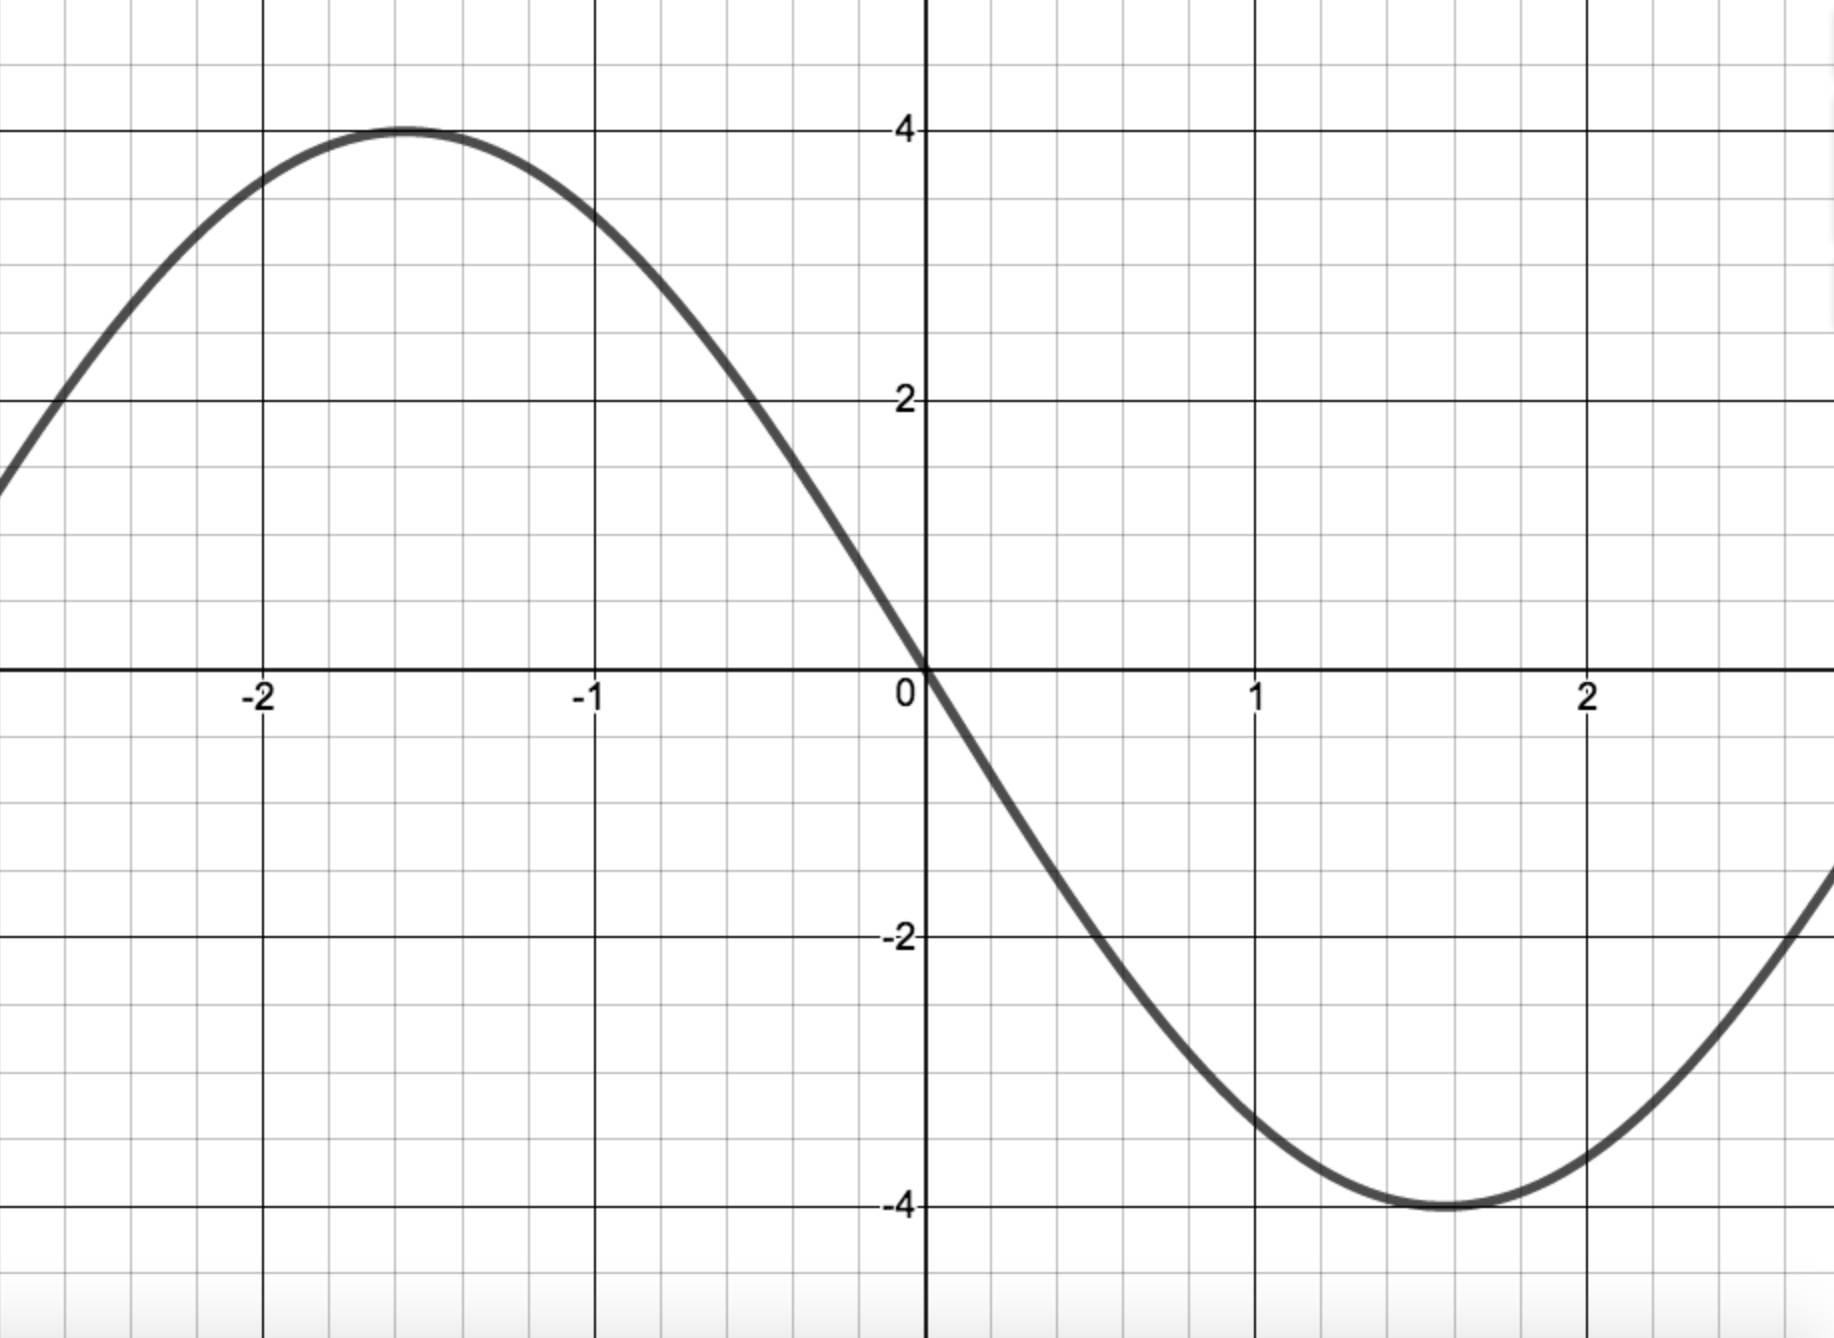
\includegraphics[width=2.75in]{./IntroductiontoDerivativesGraphics/MatchDeriv05.jpeg}

\end{multicols}

\end{center}


\newpage


\subsection{Answers}


\begin{enumerate}

\item $\ds{\lim_{h \rightarrow 0} 2 = 2}$, $\ds{\lim_{h \rightarrow 0} 2 = 2}$
\item $\ds{\lim_{h \rightarrow 0} -3 = -3}$, $\ds{\lim_{h \rightarrow 0} -3 = -3}$,

\setcounter{HW}{\value{enumi}}
\end{enumerate}

\begin{enumerate}
\setcounter{enumi}{\value{HW}}

\item $\ds{\lim_{h \rightarrow 0} 0 = 0}$,  $\ds{\lim_{h \rightarrow 0} 0 = 0}$
\item  $\ds{\lim_{h \rightarrow 0} (3h+11)= 11}$,   $\ds{\lim_{h \rightarrow 0} (6x+3h-1)= 6x-1}$

\setcounter{HW}{\value{enumi}}
\end{enumerate}

\begin{enumerate}
\setcounter{enumi}{\value{HW}}

\item    $\ds{\lim_{h \rightarrow 0} (-h-2) = -2}$,   $\ds{\lim_{h \rightarrow 0} (-2x-h+2) = -2x+2}$   
\item   $\ds{\lim_{h \rightarrow 0} (4h+16) = 16}$,   $\ds{\lim_{h \rightarrow 0} (8x+4h) = 8x}$ 

\setcounter{HW}{\value{enumi}}
\end{enumerate}

\begin{enumerate}
\setcounter{enumi}{\value{HW}}

\item \begin{itemize}  \item $f'(2) = \ds{\lim_{h \rightarrow 0} (-h-3) = -3}$

\smallskip

\item  $y = f'(2)(x-2) + f(2) = (-3)(x-2)+(-2)$ so $y  = -3x+4$.

\smallskip

\item   $f'(x) =  \ds{\lim_{h \rightarrow 0} (-2x-h+1) = -2x+1}$ 

\smallskip

\item  $y = f'(0)(x-0) + f(0) = (1)(x-0) + 0$ so $y = x$.

\smallskip

\end{itemize}

\item \begin{itemize}

\item $f'(2) = \ds{\lim_{h \rightarrow 0} \left( h^2+6h+12 \right) = 12}$

\smallskip

\item  $y = f'(2)(x-2) + f(2) = 12(x-2)+ 9$ so $y = 12x - 15$.

\smallskip

\item  $f'(x) = \ds{\lim_{h \rightarrow 0} \left(3x^{2} + 3xh + h^{2} \right) = 3x^{2}}$ 

\smallskip

\item $y = f'(0)(x-0)+f(0) = 0(x-0)+1$ so $y = 1$.

\smallskip

\end{itemize} 

\setcounter{HW}{\value{enumi}}
\end{enumerate}

\begin{enumerate}
\setcounter{enumi}{\value{HW}}

\item  $f'(x) = \ds{\lim_{h \rightarrow 0} m= m}$.

\item  \begin{itemize} \item  $f'(x) = \ds{\lim_{h \rightarrow 0} (2ax + ah + b) = 2ax + b}$.

\smallskip

\item  Solving $f'(x) = 2ax + b = 0$ for $x$ gives $x = -\frac{b}{2a}$ which is the formula for the $x$-coordinate of the vertex of the parabola $y = f(x)$.  If we zoom in near the the vertex of a parabola, the graph becomes locally flat so it makes sense the slope of the tangent line,  $f'(x) = 0$ there. 

\end{itemize} 

\setcounter{HW}{\value{enumi}}
\end{enumerate}

\begin{enumerate}
\setcounter{enumi}{\value{HW}}

\item  $\ds{ \lim_{\Delta x \rightarrow 0} \dfrac{2}{\Delta x-1} = -2}$,   $\ds{ \lim_{\Delta x \rightarrow 0} \dfrac{-2}{x(x+\Delta x)} = - \dfrac{2}{x^2}}$
 
\item  $\ds{ \lim_{\Delta x \rightarrow 0} \dfrac{-3}{2(\Delta x - 2)} = \dfrac{3}{4}}$,   $\ds{ \lim_{\Delta x \rightarrow 0} \dfrac{3}{(x+\Delta x-1)(x-1)} =  \dfrac{3}{(x-1)^2}}$  

\setcounter{HW}{\value{enumi}}
\end{enumerate}

\begin{enumerate}
\setcounter{enumi}{\value{HW}}

\item   $\ds{ \lim_{\Delta x \rightarrow 0} \dfrac{2-\Delta x}{(\Delta x - 1)^2} =2}$,   $\ds{ \lim_{\Delta x \rightarrow 0}\dfrac{-(2x+\Delta x)}{x^2(x+\Delta x)^2} =  - \dfrac{2}{x^3}}$   

\item    $\ds{ \lim_{\Delta x \rightarrow 0} \dfrac{-1}{2(\Delta x+4)} = - \dfrac{1}{8}}$,   $\ds{ \lim_{\Delta x \rightarrow 0} \dfrac{-2}{(x+5)(x+\Delta x+5)}=  - \dfrac{2}{(x+5)^2}}$    

\setcounter{HW}{\value{enumi}}
\end{enumerate}

\begin{enumerate}
\setcounter{enumi}{\value{HW}}

\item \begin{itemize}

\item  $f'(-1) =\ds{ \lim_{\Delta x \rightarrow 0} \dfrac{4}{7(4 \Delta x - 7)} = - \dfrac{4}{49}}$

\smallskip

\item $y = f'(-1)(x-(-1)) + f(-1) = -\frac{4}{49}(x + 1) + \left(-\frac{1}{7}\right)$ so $y = -\frac{4}{49} \, x - \frac{11}{49}$.   

\smallskip

\item  $f'(x) = \ds{ \lim_{\Delta x \rightarrow 0} \dfrac{-4}{(4x-3)(4x+4\Delta x-3)} =  - \dfrac{4}{(4x-3)^2}}$  

\smallskip

\item $y = f'(0)(x-0)+f(0) = -\frac{4}{9} (x-0) + \left(-\frac{1}{3}\right)$ so $y = -\frac{4}{9} \, x - \frac{1}{3}$.

\smallskip

\end{itemize}
   
\item \begin{itemize}

\item  $f'(-1) = \ds{ \lim_{\Delta x \rightarrow 0} \dfrac{6}{\Delta x + 1}= 6}$

\smallskip

\item $y = f'(-1)(x-(-1)) + f(-1) = 6(x+1) + (-3)$ so $y = 6x+3$.

\smallskip

\item  $f'(x) =\ds{ \lim_{\Delta x \rightarrow 0} \dfrac{6}{(x+2)(x+\Delta x+2)} =   \dfrac{6}{(x+2)^2}}$ 

\smallskip    

\item  $y = f'(0)(x-0) + f(0) = \frac{3}{2} \, (x-0)+0$ so $y = \frac{3}{2} \, x$.


\smallskip


\end{itemize}

 
\setcounter{HW}{\value{enumi}}
\end{enumerate}

\begin{enumerate}
\setcounter{enumi}{\value{HW}}

\item   \begin{itemize}

\item  $f'(-1) = \ds{ \lim_{\Delta x \rightarrow 0} \dfrac{9}{10(\Delta x - 10)} = -\dfrac{9}{100}}$

\smallskip

\item $y = f'(-1)(x-(-1)) + f(-1) = -\frac{9}{100} \, (x+1) + \frac{1}{10}$ so $y = - \frac{9}{100} \, x + \frac{1}{100}$.

\smallskip

\item  $f'(x) =\ds{ \lim_{\Delta x \rightarrow 0} \dfrac{-9}{(x - 9)(x + \Delta x - 9)} =   -\dfrac{9}{(x-9)^2}}$   

\smallskip  

\item  $y = f'(0)(x-0) + f(0) = -\frac{1}{9} \, (x-0)+0$ so $y = -\frac{1}{9} \, x$.

\smallskip

\end{itemize}

\item \begin{itemize}  

\item  $f'(-1) = \ds{ \lim_{\Delta x \rightarrow 0} \dfrac{\Delta x}{2 \Delta x - 1} = 0}$

\smallskip

\item $y = f'(-1)(x-(-1)) + f(-1) = (0) (x+1) + (-1)$ so $y = -1$.

\smallskip

\item  $f'(x) =\ds{ \lim_{\Delta x \rightarrow 0}\dfrac{2x^2+2x\Delta x+2x+\Delta x}{(2x+1)(2x+2\Delta x+1)}=  \dfrac{2x^2+2x}{(2x+1)^2}}$

\smallskip

\item  $y = f'(0)(x-0) + f(0) = (0)(x-0)+0$ so $y = 0$.

\smallskip

\end{itemize}


\setcounter{HW}{\value{enumi}}
\end{enumerate}

\begin{enumerate}
\setcounter{enumi}{\value{HW}}

\item  $\ds{ \lim_{\Delta t \rightarrow 0}\dfrac{-1}{\sqrt{9-\Delta t} +3}  = -\dfrac{1}{6}}$,   $\ds{ \lim_{\Delta t \rightarrow 0} \dfrac{-1}{\sqrt{9-t-\Delta t} + \sqrt{9-t}}=   -\dfrac{1}{2 \sqrt{9-t}}}$   
\item  $\ds{ \lim_{\Delta t \rightarrow 0}\dfrac{2}{\sqrt{2\Delta t+1} + 1}  =1}$,   $\ds{ \lim_{\Delta t \rightarrow 0}\dfrac{2}{\sqrt{2t+2\Delta t+1} + \sqrt{2t+1}}=   \dfrac{2}{2 \sqrt{2t+1}}}$    

\setcounter{HW}{\value{enumi}}
\end{enumerate}

\begin{enumerate}
\setcounter{enumi}{\value{HW}}

\item \begin{itemize}

\item  $g'(0) = \ds{ \lim_{\Delta t \rightarrow 0} \dfrac{-4}{\sqrt{5-4\Delta t} + \sqrt{5}}  = - \dfrac{2}{\sqrt{5}}}$

\smallskip

\item  $y = g'(0) (x - 0) + g(0) =  -\frac{2}{\sqrt{5}} \, (x-0) + \sqrt{5}$ so $y = -\frac{2}{\sqrt{5}} \, x + \sqrt{5}$.

\smallskip

\item  $g'(t) =  \ds{ \lim_{\Delta t \rightarrow 0} \dfrac{-4}{\sqrt{-4t-4\Delta t+5} + \sqrt{-4t+5}} =   -\dfrac{2}{\sqrt{-4t+5}}}$

\smallskip

\item  $y = g'(1)(x-1)+g(1) = (-2)(x-1) + 1$ so $y = -2x+3$.

\smallskip

\end{itemize}

\item   \begin{itemize}

\item  $g'(0) = \ds{ \lim_{\Delta t \rightarrow 0} \dfrac{-1}{\sqrt{4-\Delta t} + 2}  = - \dfrac{1}{4}}$

\smallskip

\item  $y = g'(0) (x - 0) + g(0) =  -\frac{1}{4} \, (x-0) + 2$ so $y = -\frac{1}{4} \, x +2$.

\smallskip

\item  $g'(t) = \ds{ \lim_{\Delta t \rightarrow 0} \dfrac{-1}{\sqrt{4-t-\Delta t} + \sqrt{4-t}} = -\dfrac{1}{2 \sqrt{4-t}} }$  

\smallskip

\item  $y = g'(1)(x-1)+g(1) = -\frac{1}{2 \sqrt{3}} \, (x-1) + \sqrt{3}$ so $y =  -\frac{1}{2 \sqrt{3}}  \, x + \frac{7 \sqrt{3}}{6}$.

\smallskip

\end{itemize}


\item   \begin{enumerate}

\item  If $\Delta t < 0$, then $\sqrt{\Delta t}$ is not a real number.  Hence, $g'(0) = \ds{\lim_{\Delta t \rightarrow 0} \dfrac{g(\Delta t) - g(0)}{\Delta t}}$ does not exist.

\item  $g_{+}'(0) =\ds{ \lim_{\Delta t \rightarrow 0^{+}} (\Delta t)^{\frac{1}{2}}   =  0}$

\smallskip

\item  $y = g_{+}'(0) (x - 0) + g(0) =  (0) (x-0) + 0$ so $y = 0$.  

\smallskip

This line is a tangent line to the graph of $y = t \sqrt{t}$ at $(0,0)$ for $t \geq 0$.

\smallskip

\item  $g'(t) =\ds{ \lim_{\Delta t \rightarrow 0}\dfrac{3t^2+3t\Delta t+(\Delta t)^2}{(t+\Delta t)^{3/2} + t^{3/2}} = \dfrac{3t^2}{2 t^{3/2}} = \dfrac{3}{2} \, t^{1/2}}$ provided $t > 0$.


\end{enumerate}


\setcounter{HW}{\value{enumi}}
\end{enumerate}

\begin{enumerate}
\setcounter{enumi}{\value{HW}}

\item  \begin{enumerate} \item  $g'(t) = \ds{ \lim_{\Delta t \rightarrow 0} \dfrac{a}{\sqrt{at+a\Delta t+b} + \sqrt{at+b}} = \dfrac{a}{2 \sqrt{at+b}} }$.  

\smallskip

\item  We are told $a \neq 0$.  In order for the square roots to be happy, we assume $at + b > 0$.  Hence,   $t >  - \frac{b}{a}$ if $a>0$ and $t < -  \frac{b}{a}$ if $a<0$. 

\end{enumerate}

\setcounter{HW}{\value{enumi}}
\end{enumerate}


\begin{enumerate}
\setcounter{enumi}{\value{HW}}

\item \begin{enumerate} \item  $f$ is continuous at $x=0$ since $\ds{\lim_{x \rightarrow 0} f(x) = \lim_{x \rightarrow 0} |x| = 0 = |0| = f(0)}$.

\smallskip

\item   $\ds{\lim_{h \rightarrow 0^{-}} \dfrac{f(h) - f(0)}{h} = \lim_{h \rightarrow 0^{-}} \dfrac{-h}{h}  =-1}$,  $\ds{\lim_{h \rightarrow 0^{+}} \dfrac{f(h) - f(0)}{h} = \lim_{h \rightarrow 0^{+}} \dfrac{h}{h}  = 1}$

\smallskip
        
\item  Near $x = 0$, the graph of $y = f(x)$ looks like a `$\vee$' shape\footnote{We say the graph of $f$ has a  \index{corner}\textbf{corner} at $(0,0)$ since we have two different, but finite slopes meeting at a point.} consisting of a line of slope $-1$ to the left of $x=0$ and a line with a slope of $+1$ to the right of $x = 0$.

\smallskip

\item  $f'(x) =  \ds{\lim_{h \rightarrow 0} \dfrac{|x+h| - |x|}{h} = -1}$ if $x < 0$ and $f'(x) =  \ds{\lim_{h \rightarrow 0} \dfrac{|x+h| - |x|}{h} = 1}$ of $x > 0$.

\smallskip

\end{enumerate}



\item \begin{enumerate}

\item  $g$ is continuous at $t=0$ since $\ds{\lim_{t \rightarrow 0} g(t) = \lim_{t \rightarrow 0} \sqrt[3]{t} = 0 = \sqrt[3]{0} = g(0)}$.

\smallskip

\item $\ds{\lim_{\Delta t \rightarrow 0} \dfrac{g(\Delta t) - g(0)}{\Delta t} =   \lim_{\Delta t \rightarrow 0} \dfrac{1}{(\Delta t)^{\frac{2}{3}}}   =  \infty}$

\smallskip

        
\item  The graph of $y = g(t)$ near $(0,0)$ is a vertical line.\footnote{We say the graph of $g$ has a  \index{vertical tangent}\index{tangent line ! vertical}\textbf{vertical tangent line} at $(0,0)$.  This is the more formal way to describe all of the `unusual steepness' we saw back in Chapter \ref{RootRadicalPowerFunctions}.}  Since $g$ is increasing through $(0,0)$, the `slope' of this vertical line could be seen as $+ \infty$. 

\smallskip

\item   $g'(t) = \ds{ \lim_{\Delta t \rightarrow 0} \dfrac{1}{(t+\Delta t)^{\frac{2}{3}} + (t+\Delta t)^{\frac{1}{3}} t^{\frac{1}{3}} + t^{\frac{2}{3}}} = \dfrac{1}{3 t^{\frac{2}{3}}} }$, $t \neq 0$.

\end{enumerate}

\item \begin{enumerate}  \item $\ds{\lim_{x \rightarrow 0} h(x) = \lim_{x \rightarrow 0} x^{\frac{2}{3}} = 0 = 0^{\frac{2}{3}} = h(0)}$. 

\item $\ds{\lim_{\Delta x \rightarrow 0^{-}} \dfrac{h(\Delta x) - h(0)}{\Delta x} = \lim_{\Delta x \rightarrow 0^{-}} \dfrac{1}{(\Delta x)^{\frac{1}{3}}} = -\infty}$ and  $\ds{\lim_{\Delta x \rightarrow 0^{+}} \dfrac{h(\Delta x) - h(0)}{\Delta x} = \lim_{\Delta x \rightarrow 0^{+}} \dfrac{1}{(\Delta x)^{\frac{1}{3}}} = \infty}$

\smallskip
        
\item  The graph $y = h(x)$ near $(0,0)$ shows a steeply decreasing graph as we approach $(0,0)$ from the left followed by a steeply increasing graph as we approach $(0,0)$ from the right.\footnote{We say the graph of $f$ has a  \index{cusp}\textbf{cusp} at $(0,0)$ since we have two different, infinite slopes meeting at a point.}

\smallskip

\item  $h'(x) =  \ds{\lim_{\Delta x \rightarrow 0} \dfrac{h(x+\Delta x) - h(x)}{\Delta x} = \lim_{\Delta x \rightarrow 0} \dfrac{2x + \Delta x}{(x+\Delta x)^{\frac{4}{3}} + (x+\Delta x)^{\frac{2}{3}} \, x^{\frac{2}{3}} + x^{\frac{4}{3}}} = \dfrac{2}{3x^{\frac{1}{3}}}}$, $x \neq 0$.
\end{enumerate}

\item  \begin{enumerate}

\item  $v(t) = \ds{\lim_{\Delta t \rightarrow 0} \dfrac{h(t + \Delta t) - h(t)}{\Delta t} = \lim_{\Delta t \rightarrow 0} \dfrac{-16(\Delta t)^2 -32 t \, \Delta t + 22.08 \Delta t}{\Delta t}  = -32t + 22.08}$.

\item   $v(0) = -32(0) + 22.08 = 22.08$. This means initially (when Jason lets go of the hammer), the hammer is traveling upwards at $22.08$ feet per second.

\item  $v(t) = 0$  when $t = \frac{22.08}{32} = 0.69$.  This means the (vertical) velocity zeros out $0.69$ seconds after Jason lets go of the hammer.  In this scenario, this corresponds to when the hammer reaches its peak height

\item  We first find when the hammer hits the ground by solving $h(t) = 0$.  The positive answer here is   $t \approx 1.612$ seconds.  The velocity of the hammer is:  $v(1.612) = -32(1.612) + 22.08 = -29.504$.  The hammer hits the ground going (approximately) $29.504$ feet per second.\footnote{The negative `$-$' here on $v(1.612)$ indicates the hammer is heading \textbf{downwards} when it strikes the ground.}

\end{enumerate}

\item  \begin{enumerate}  \item  $F'(t) = \ds{\lim_{h \rightarrow 0} \dfrac{F(t + h) - F(t)}{h} = \lim_{h \rightarrow 0} \dfrac{-0.0076h^{2} -0.0152th+0.45h}{h} =-0.0152t + 0.45}$.

\item   $F'(0) = 0.45$, so fuel economy was increasing at a rate of $0.45$ mpg per year in 1980.\footnote{Since the domain of $F$ is $0 \leq t \leq 28$, $F'(0)$ is actually $F_{+}'(0)$.}

\smallskip

 $F'(5) = 0.374$,  so fuel economy was increasing at a rate of $0.374$ mpg per year in 1985. 
 
 \smallskip
 
  $F'(10) = 0.298$,  so fuel economy was increasing at a rate of $0.298$ mpg  per year in 1990. 

\item  Based on the model, we have that during the years 1980 - 1990, fuel economy was increasing, but less so as the decade wore on.  Technical and cost limitations could be at work here.

\end{enumerate}

\item   \begin{enumerate}  \item   $C'(75) = \ds{\lim_{h \rightarrow 0} \dfrac{C(75+h) - C(75)}{h}  =     \lim_{h \rightarrow 0} \dfrac{0.03h^{3}+2.25h^{2}+56.25h}{h} = 56.25}$.  This means when producing 75 systems, the cost is increasing at a rate of $\$ 56.25$ per system.

\item  We see that $C'(75)$ is numerically close to $MC(75)$ but the former is a rate of change (measured in dollars per system) where the latter is a change (measured in dollars).  Note that if we set  $h = 1$ in the difference quotient:  \[\dfrac{C(75+h) - C(75)}{h} = \dfrac{C(75+1) - C(75)}{1} = C(76) - C(75)\] we see these two quantities can be used to approximate each other.

\end{enumerate}

\setcounter{HW}{\value{enumi}}
\end{enumerate}





\begin{multicols}{3}

\begin{enumerate}
\setcounter{enumi}{\value{HW}}

 \item $f'(x)$ is Graph B
 
 \item $g'(x)$ is Graph C
 
 
 \item $h'(x)$ is Graph A 

\setcounter{HW}{\value{enumi}}
\end{enumerate}

\end{multicols}


\begin{multicols}{3}

\begin{enumerate}
\setcounter{enumi}{\value{HW}}

 \item $f'(x)$ is Graph B
 
 \item $g'(x)$ is Graph A
 
 \item $h'(x)$ is Graph C

\setcounter{HW}{\value{enumi}}
\end{enumerate}

\end{multicols}






\begin{itemize}

\item  difference quotients

\item velocities

\item other rates of change (marginals?)

\item  tangent lines

\item  derivative formulas: constant, linear,  quadratic

\item foreshadow inc / dec

\item  vertex formula (reprise)


\end{itemize}

\closegraphsfile
